\documentclass[12pt,a4paper]{style}

%%%%%%%%% Preamble

% used for figures:
\usepackage{graphicx}
% math fonts etc.:
\usepackage{amsmath,amsfonts,amsthm,latexsym,amssymb}
\usepackage{pdfpages}
\usepackage{caption,subcaption}
\usepackage{hyperref}
\hypersetup{
	colorlinks,
	citecolor=black,
	filecolor=black,
	linkcolor=blue,
	urlcolor=black
}
\usepackage{wrapfig}
\setlength\intextsep{2pt} % avoid too much space around figure (can be set to 0pt at maximum)

\graphicspath{ {figures/} }
%%%%%%%%%%

\begin{document}
	\tableofcontents
	\listoffigures
	\newpage
	\begin{center}
		\textcolor{orange}{\Large {\bf{ShowTime OTT service case study}}}
	\end{center}
	
\section{Business context}
OTT (Over-the-Top) media services deliver content directly to viewers via the internet, bypassing traditional TV. These platforms, offering on-demand video and music, are becoming increasingly popular due to their convenience and better digital connectivity. The global OTT market, valued at \$121.61 billion in 2019, is projected to reach \$1,039.03 billion by 2027, growing rapidly at a 29.4\% CAGR. The shift from traditional broadcasting to OTT services has accelerated, especially during the COVID-19 pandemic, which saw a 46\% increase in consumption. Ongoing innovations in OTT platforms are expected to further attract and retain subscribers globally.
ShowTime is a growing OTT company. To address the current objectives, our focus is on identifying the key drivers of first-day content viewership. By understanding these factors, we can implement strategies to enhance viewer engagement on the platform. Possible reasons for the recent decline in viewership include decreased platform traffic, reduced marketing investments, scheduling conflicts, and variations due to weekends and holidays.

In our role as Data Scientists for ShowTime company, we will analyze the data to develop a linear regression model. This model will help us uncover the significant factors influencing first-day viewership and provide actionable insights to improve content performance and platform engagement.
\section{Exploratory data analysis}
\subsection{Data set description}
\begin{wrapfigure}{R}{0.65\textwidth}
	\vspace{-1mm} % move picture up
	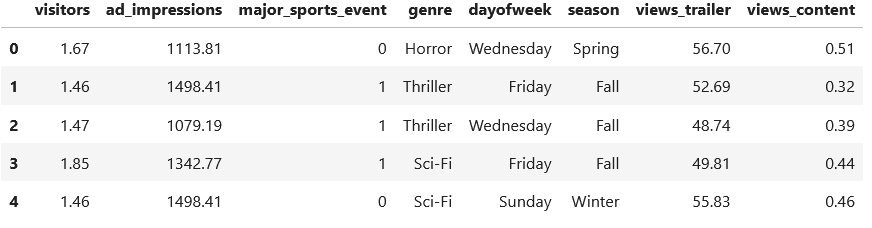
\includegraphics[width=0.65\textwidth]{dataset.png}
	\vspace{-4mm} % spacing between figure and caption
	\caption{A snapshot of data set used for analysis.}
	\label{fig:dataset}
\end{wrapfigure}
We have been provided with a content views record for each show released. The data set which we have used to generate this report has following features. visitors : which is a numerical variable for number of customers in millions that engaged in the platform past week prior to show release. Ad impressions : a numerical variable for number of ads invested in millions across all ad campaigns for the content both running and completed. Major sports event : a categorical variable having values 0 or 1 to show whether on the day of release there was a major sports event. Genre : the category of show released for e.g Scifi, action, romance etc. Day of week : a string field for the day of release of the content. Season : in which season the content was released. Trailer views : a numerical variable for number of views in millions of the content trailer prior to show released. Lastly content views : a numerical variable for the number of first-day views in millions of the content. Figure \ref{fig:dataset} shows a snap shot of the data set used in this analysis. In total we have 8 columns/fields and 1000 records/rows.    

 Our aim is to study these variables and find any relationship between these variables or some pattern to give us business insights and help us with strengthening business strategies. One of the most important aspect of data analysis is making sure that we have valid data set. For this we perform data cleaning and look for any irregularities and outliers in the data set which can negatively impact our analysis. Fortunately we did not find any missing or null values in our data set. No duplicated records were found. We checked unique values for each categorical variables and we did not find any irregularities or typos. To have a idea about outliers in our data set we have checked  boxplots for each numerical variables. We observed that there are presence of many outliers. figure \ref{fig:outlier} shows box plot for trailer and content views. But we did not treat or remove these outliers as all the records are a valid observations corresponding to some show release. 
 \begin{figure}
 	\centering
 	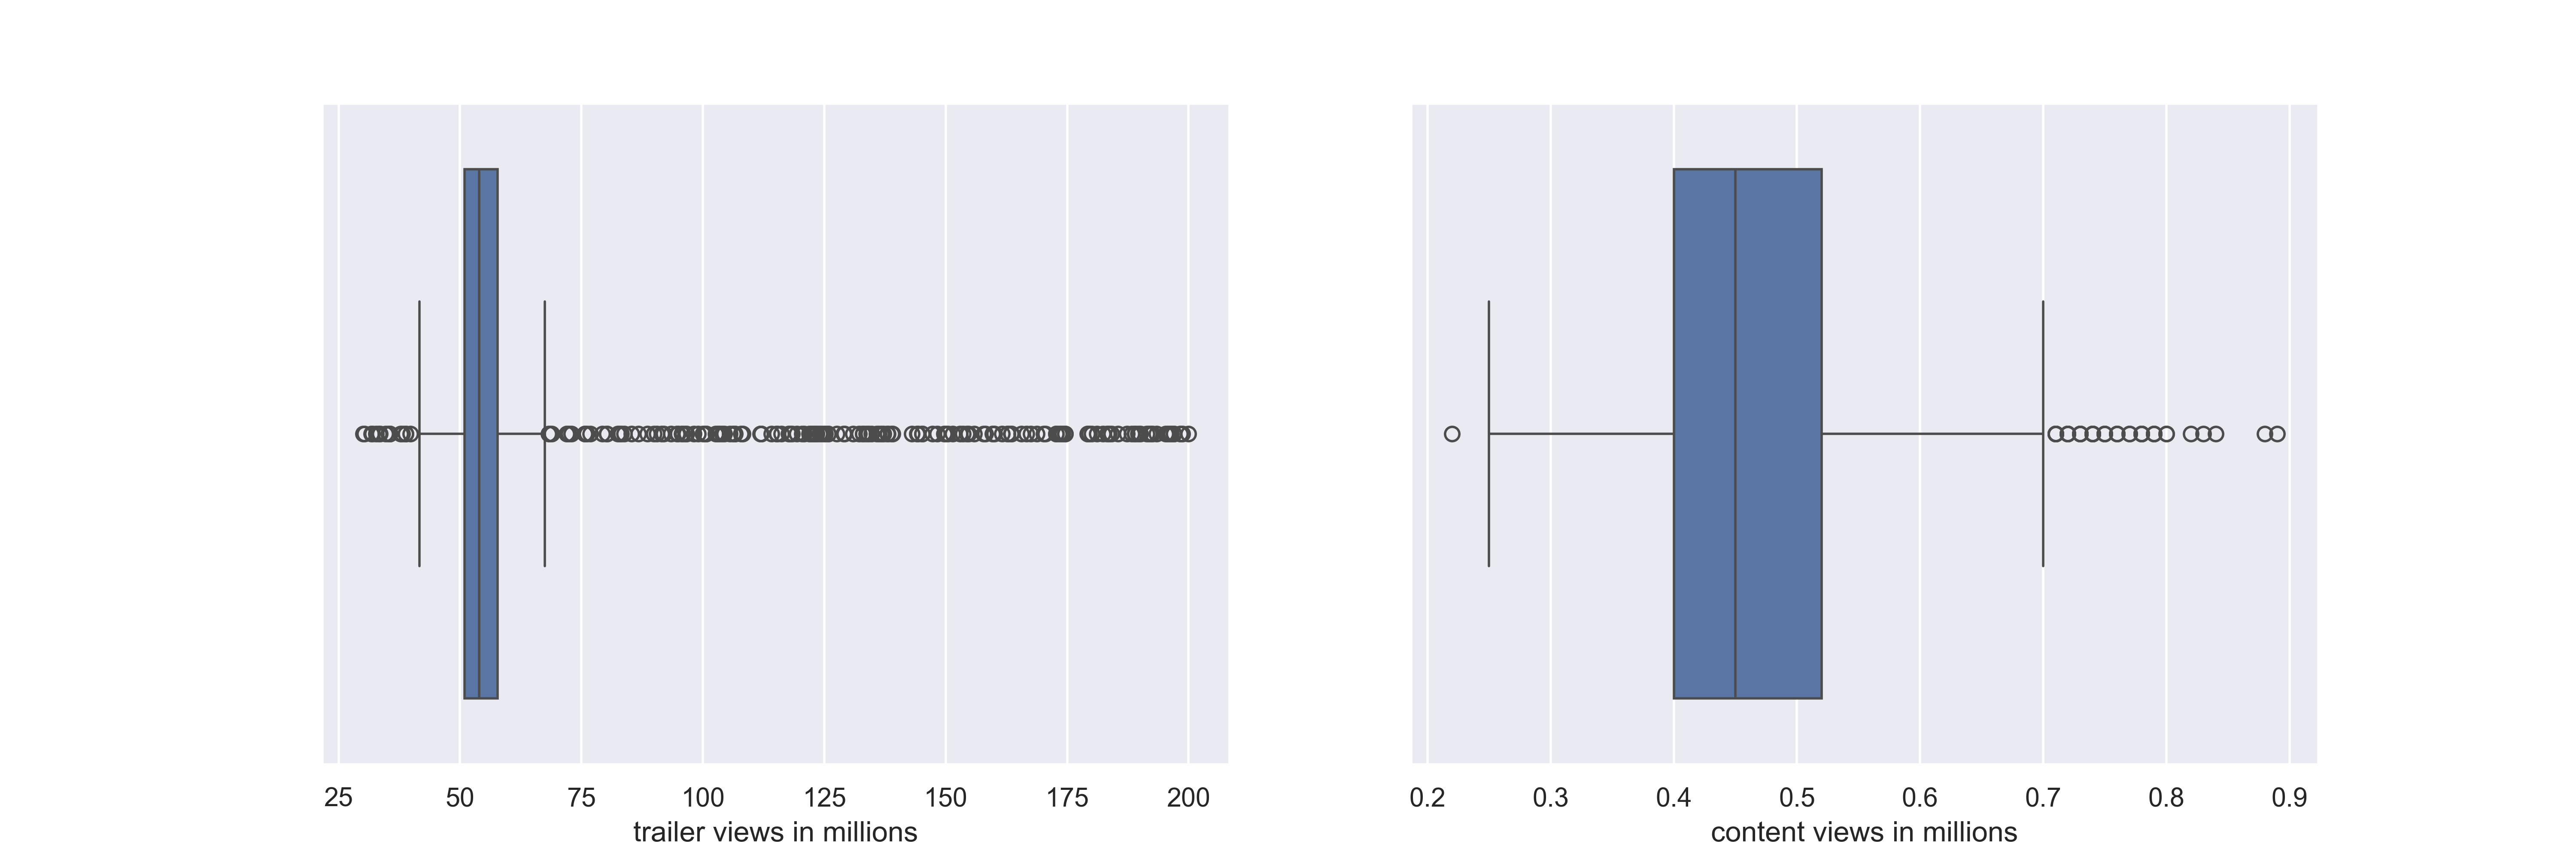
\includegraphics[width=\textwidth]{outlier.png}
 	\caption{Box plot for trailer views(left) and content views(right). }
 	\label{fig:outlier}
 \end{figure}
\subsection{What does the distribution of content views look like?}
In the analysis we have studied distribution of all the numerical as well as categorical values which is important to find any irregularities or bias in the data set. Figure \ref{fig: Distribution of numerical variables } shows plot for distribution of all numerical variables. We observe that number of visitors to the platform prior to show release vary from 1.2 million to 2.2 million with a mean visit of 1.7 millions. The distribution is shown in figure \ref{fig:visit distribution}. The distribution for number of ad impressions invested is shown in figure \ref{fig:ad_impression distribution}. Figure \ref{fig:trailer_views dist} shows the trailer views distribution where we find there is a strong peak around 60 million views. The plot looks like a vary narrow normal distribution. But there are many outliers and data has strong spread to right up to 200 million views. Figure \ref{fig: content_views dist} shows distribution of content views. It roughly looks like a normal distribution but with right skewness. The values vary from 0.2 to 0.9 million views with a mean of 0.47 million and a standard deviation of 0.1 million.		  
\begin{figure}[h]
	\centering
	\begin{subfigure}[t]{0.49\textwidth}
		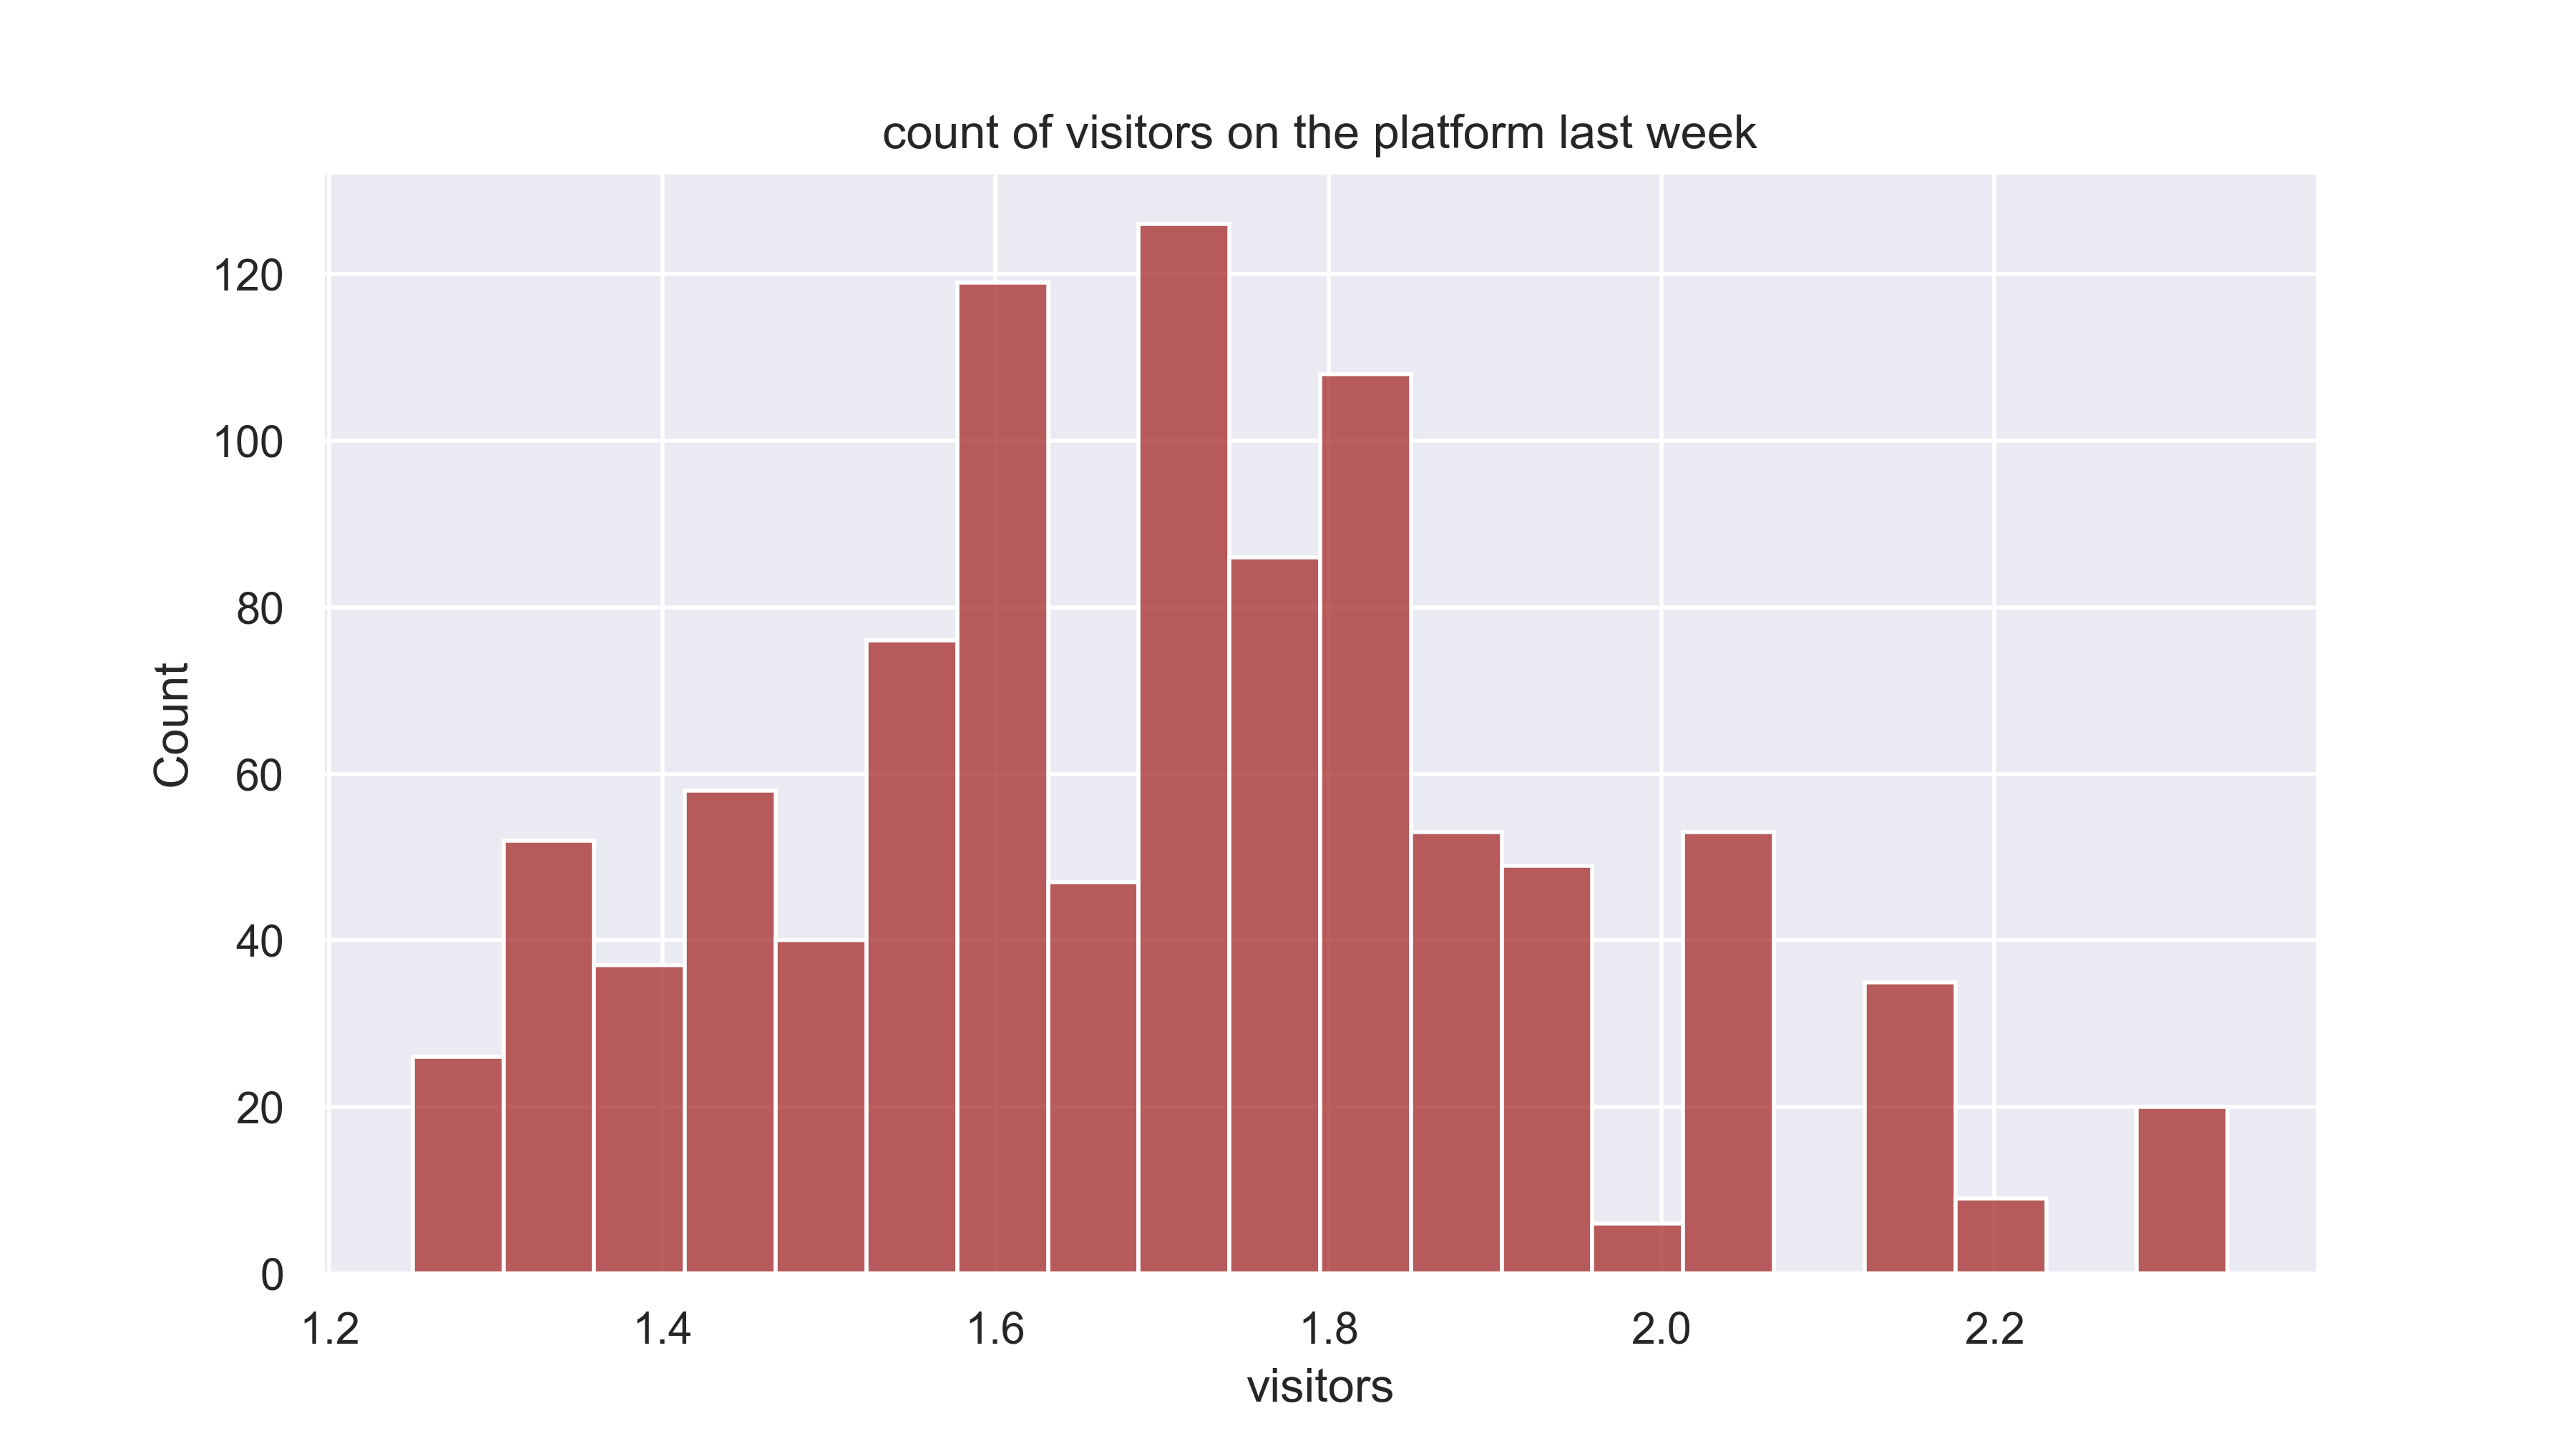
\includegraphics[width=\textwidth]{visit_dist.png}
		\caption{}
		\label{fig:visit distribution}
	\end{subfigure}
	\hfill
	\begin{subfigure}[t]{0.49\textwidth}
		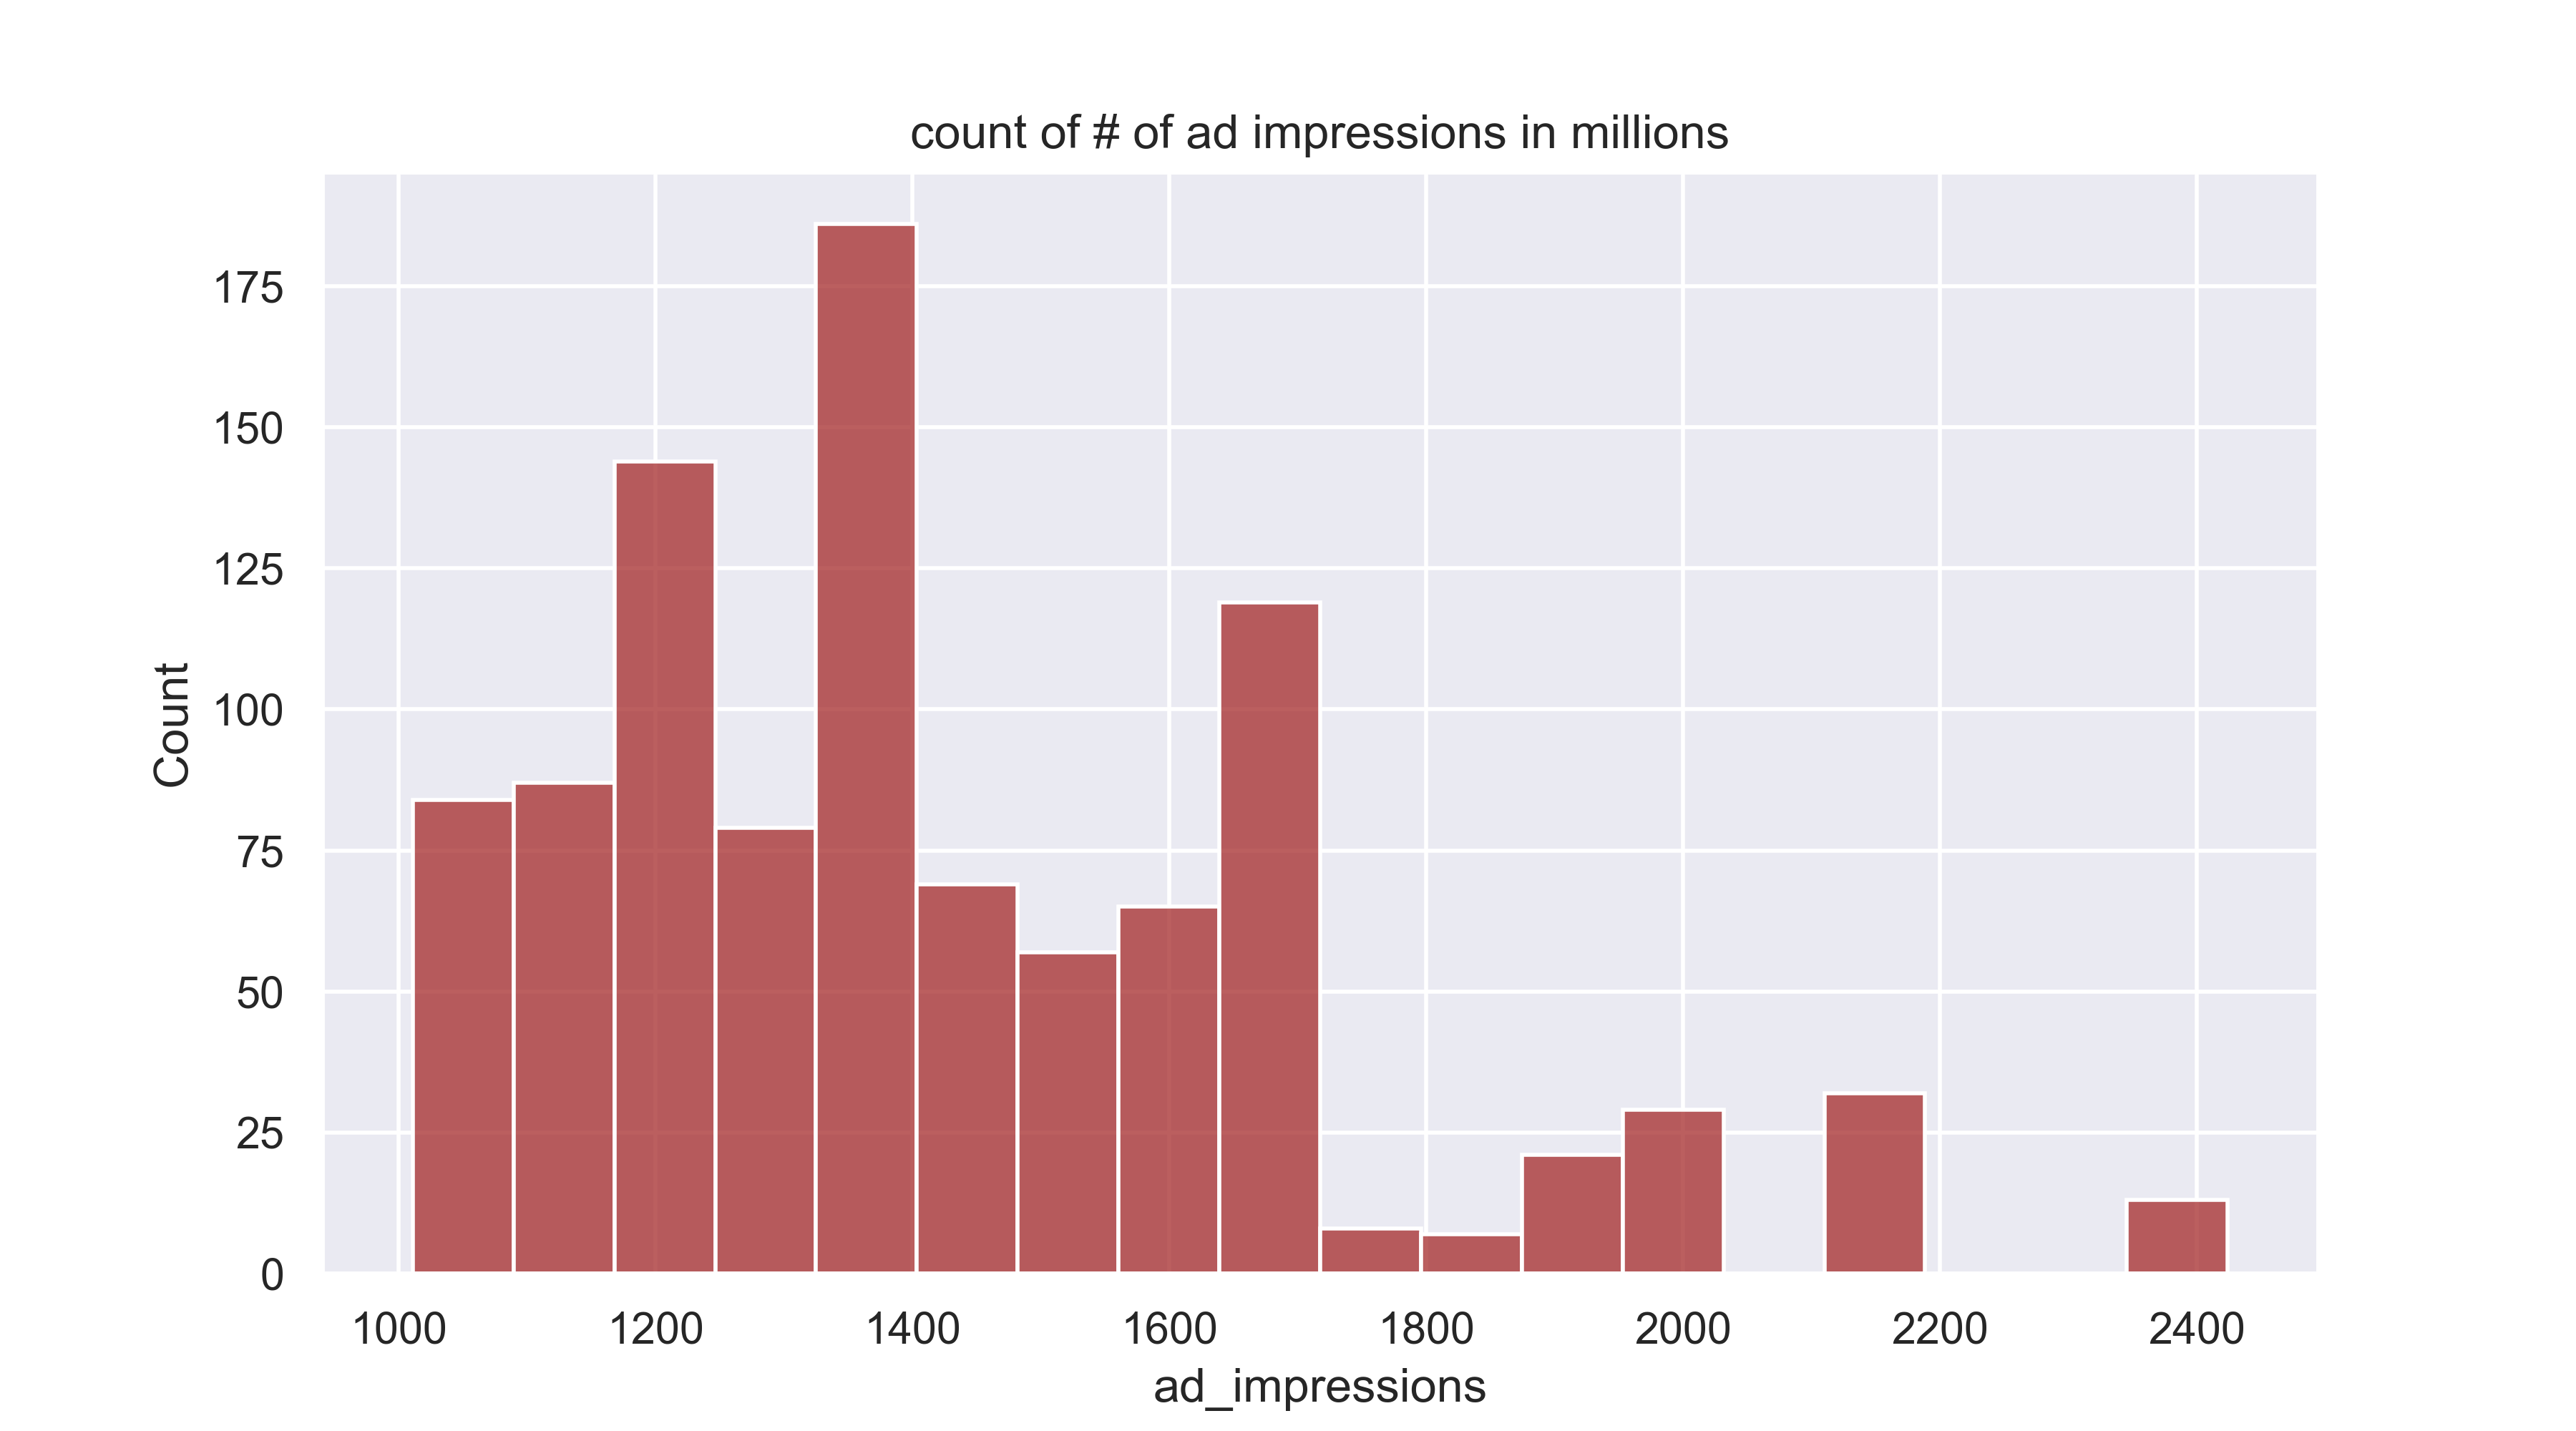
\includegraphics[width=\textwidth]{adimpressions_dist.png}
		\caption{}
		\label{fig:ad_impression distribution}
	\end{subfigure}
	\begin{subfigure}[t]{0.49\textwidth}
	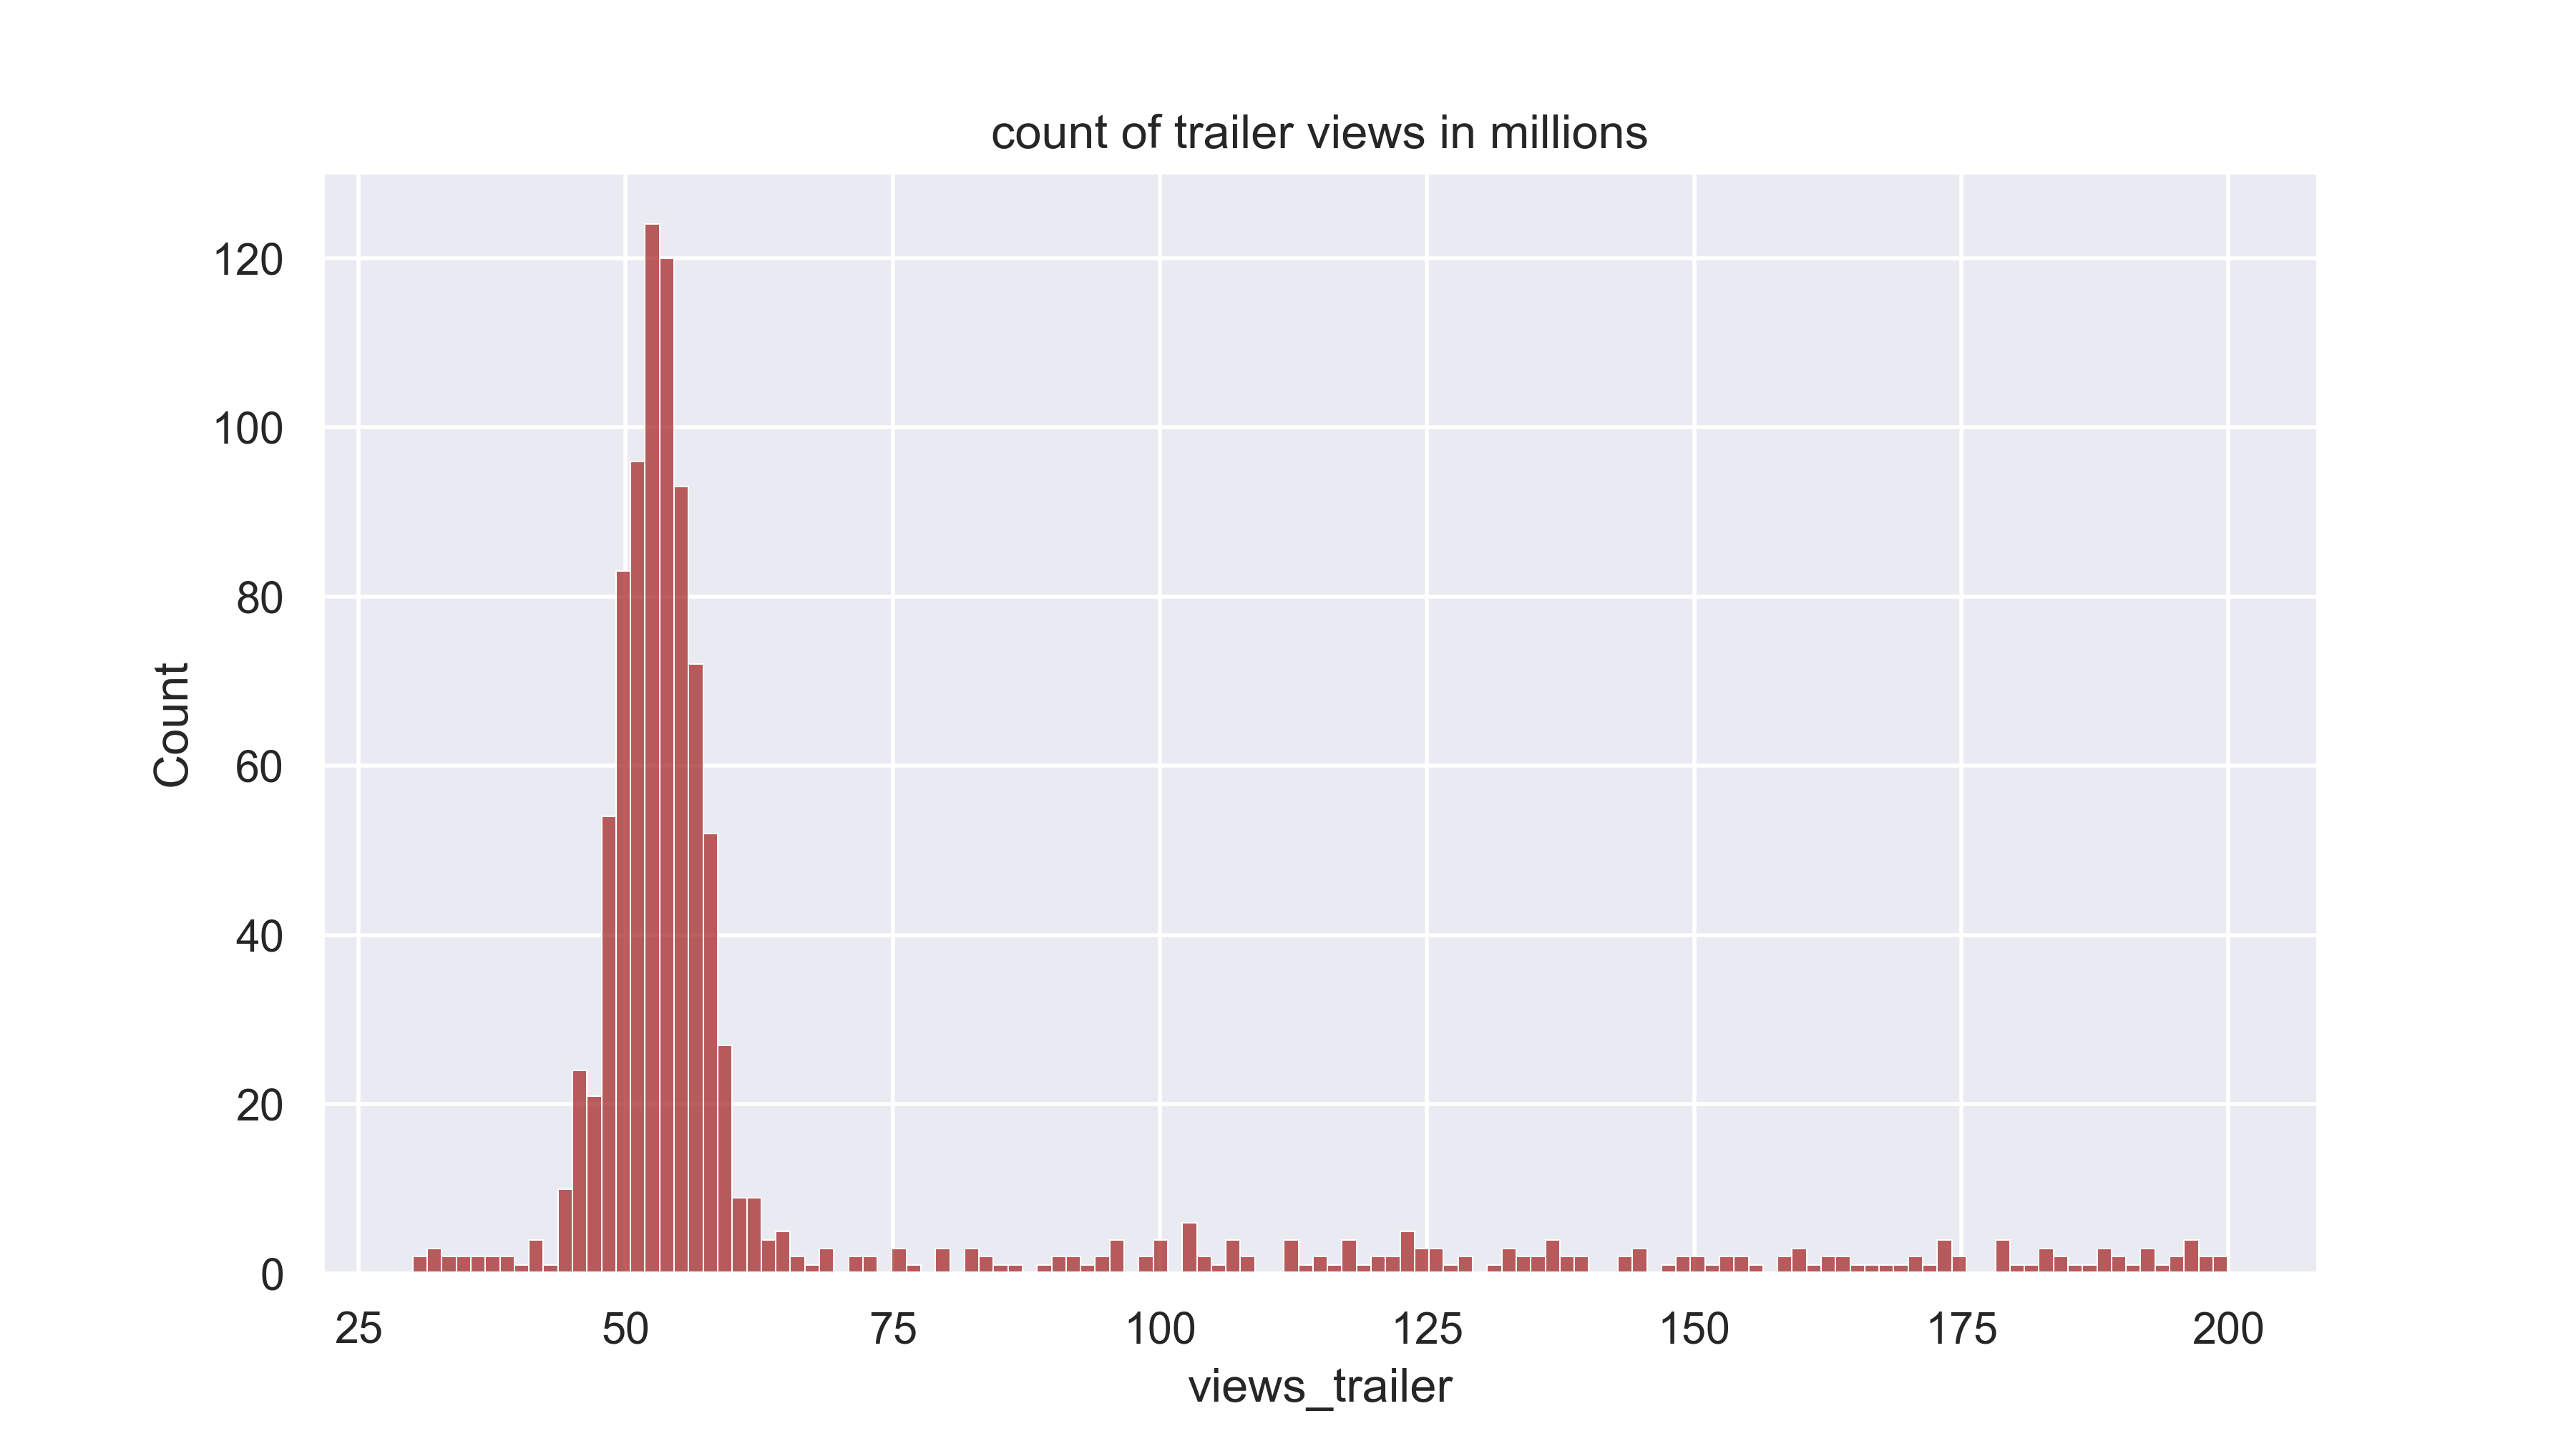
\includegraphics[width=\textwidth]{trailer_views_dist.png}
	\caption{}
	\label{fig:trailer_views dist}
	\end{subfigure}
	\hfill
	\begin{subfigure}[t]{0.49\textwidth}
	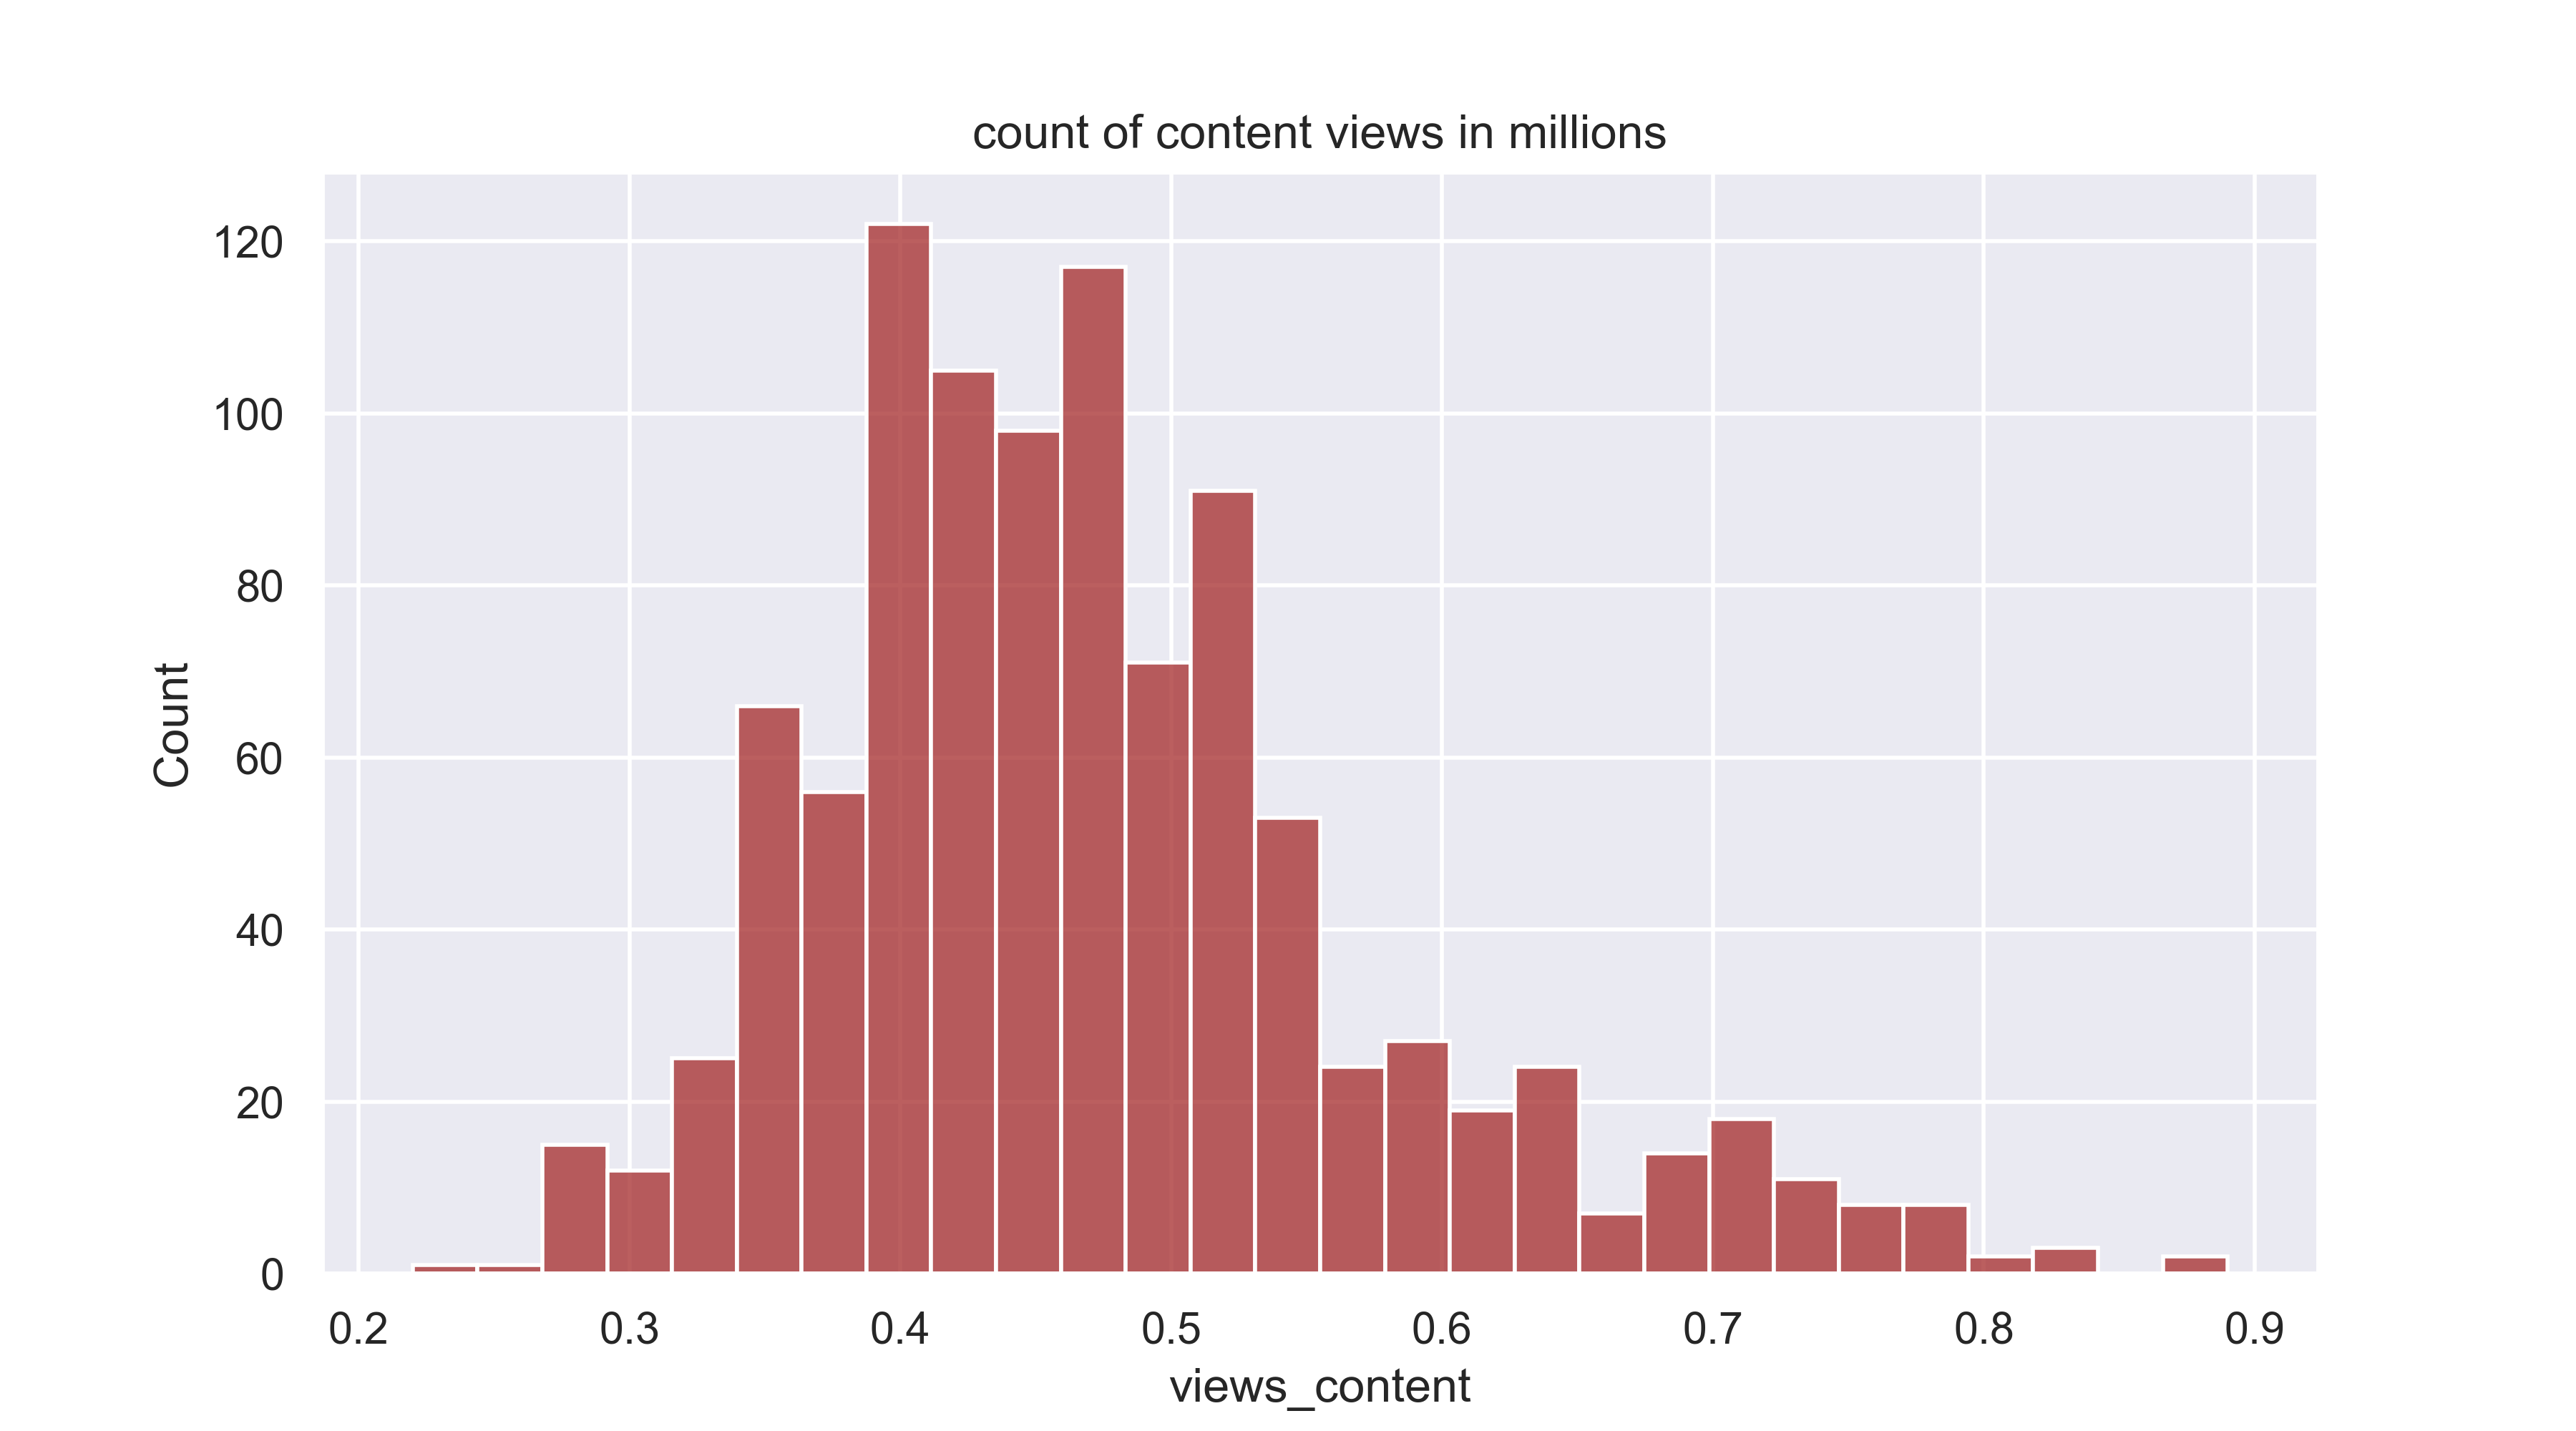
\includegraphics[width=\textwidth]{content_views_dist.png}
	\caption{}
	\label{fig: content_views dist}
	\end{subfigure}
	\caption{Distribution of numerical variables}
	\label{fig: Distribution of numerical variables }
\end{figure}

\subsection{What does the distribution of genres look like?}
Figure \ref{fig:genre and day dist} shows distribution of genre of show released and the day of week on which show released for our data set. We observe in figure \ref{fig:genre dist}that all the genres have roughly same number of shows around 100 in our data set. This is a positive factor for our analysis as we don't want the distribution in our data set to get biased towards any particular genre. In figure \ref{fig:dayofweek dist} we find that more than 60\% of the shows are released on Friday and Wednesday. 
\begin{figure}[h]
	\centering
	\begin{subfigure}[t]{0.49\textwidth}
		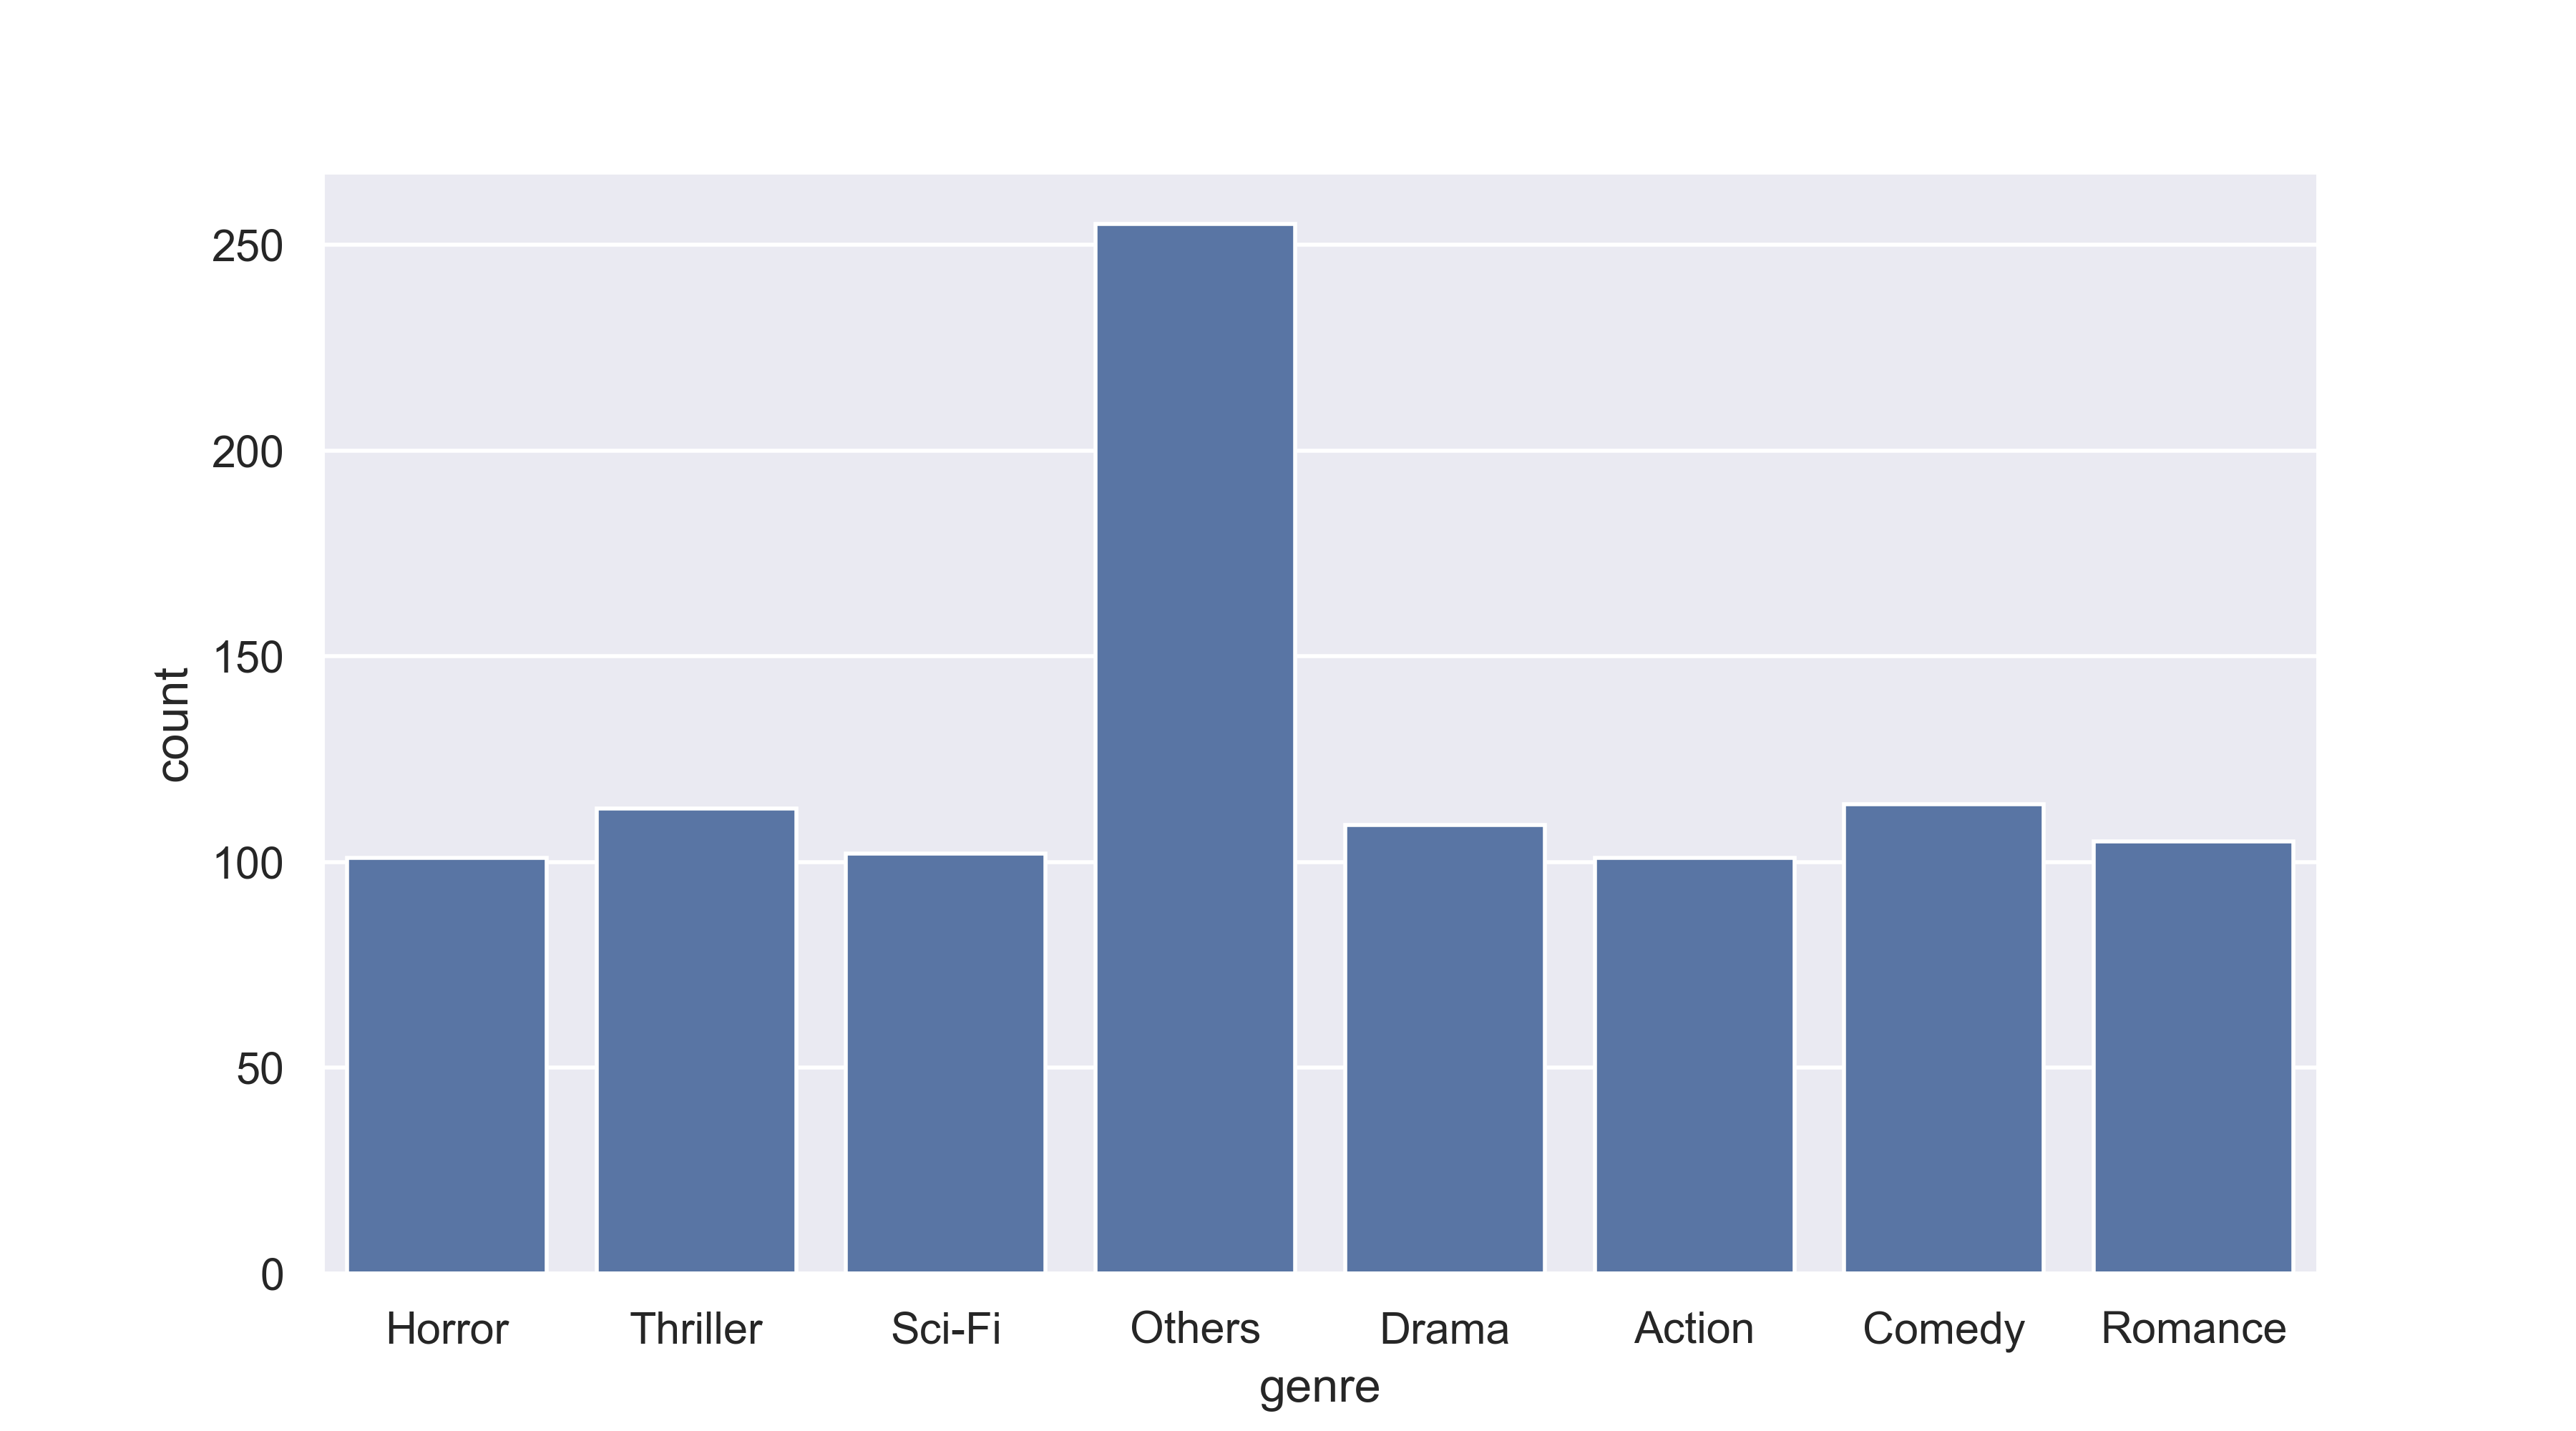
\includegraphics[width=\textwidth]{genre_dist.png}
		\caption{}
		\label{fig:genre dist}
	\end{subfigure}
	\hfill
	\begin{subfigure}[t]{0.49\textwidth}
		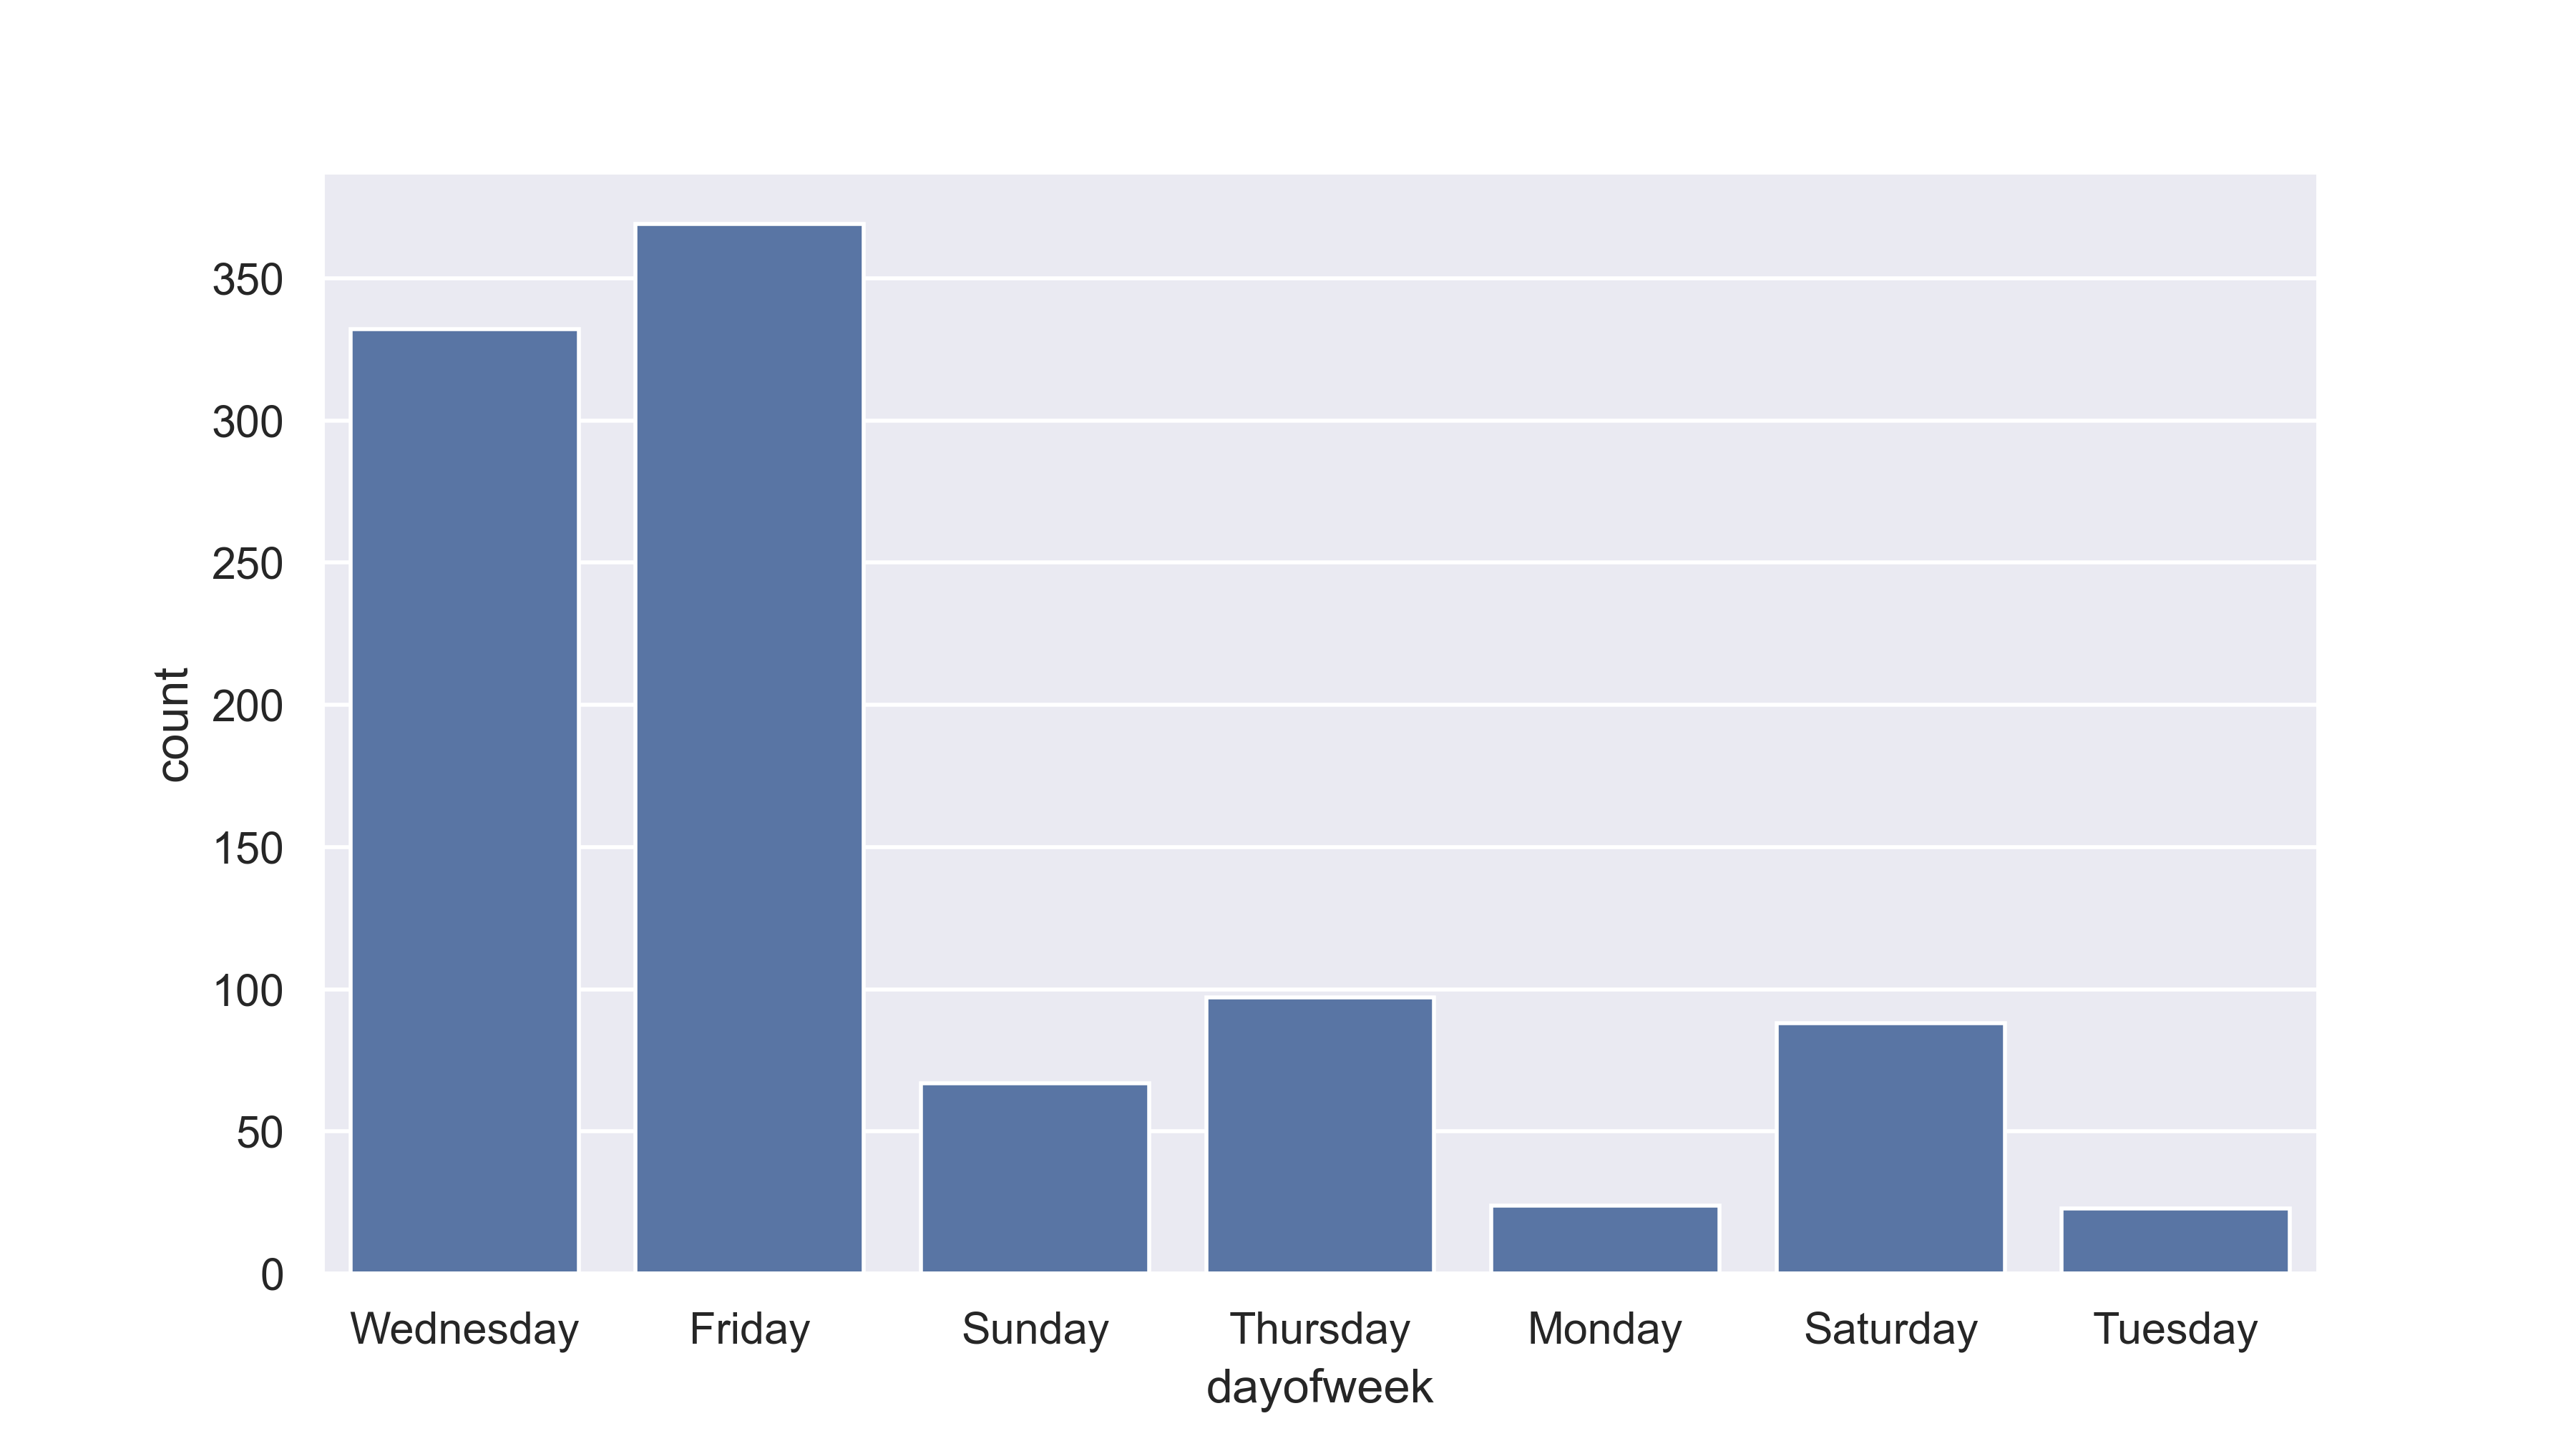
\includegraphics[width=\textwidth]{dayofweek.png}
		\caption{}
		\label{fig:dayofweek dist}
	\end{subfigure}
	\caption{Distribution of genre and day of week release.}
	\label{fig:genre and day dist}
\end{figure}

\subsection{How does the viewership vary with the season and day of release?}
Figure \ref{fig:day and season effect} we have plotted box plot for content views with respect to day of week and season on which the show is released. We observe that shows released on Saturday has highest median first day viewership. But as shown in figure \ref{fig:content_views_vs_dayofweek}, it is worth while to note that all the box plots have outliers and the difference with respect to day of release is not big. most of them have median values around 0.45 million views. Figure \ref{fig:content_views_vs_season} shows content views distribution with respect to seasons. Shows released in summer have highest number of median first day views. 
\begin{figure}
	\centering
	\begin{subfigure}[t]{0.49\textwidth}
		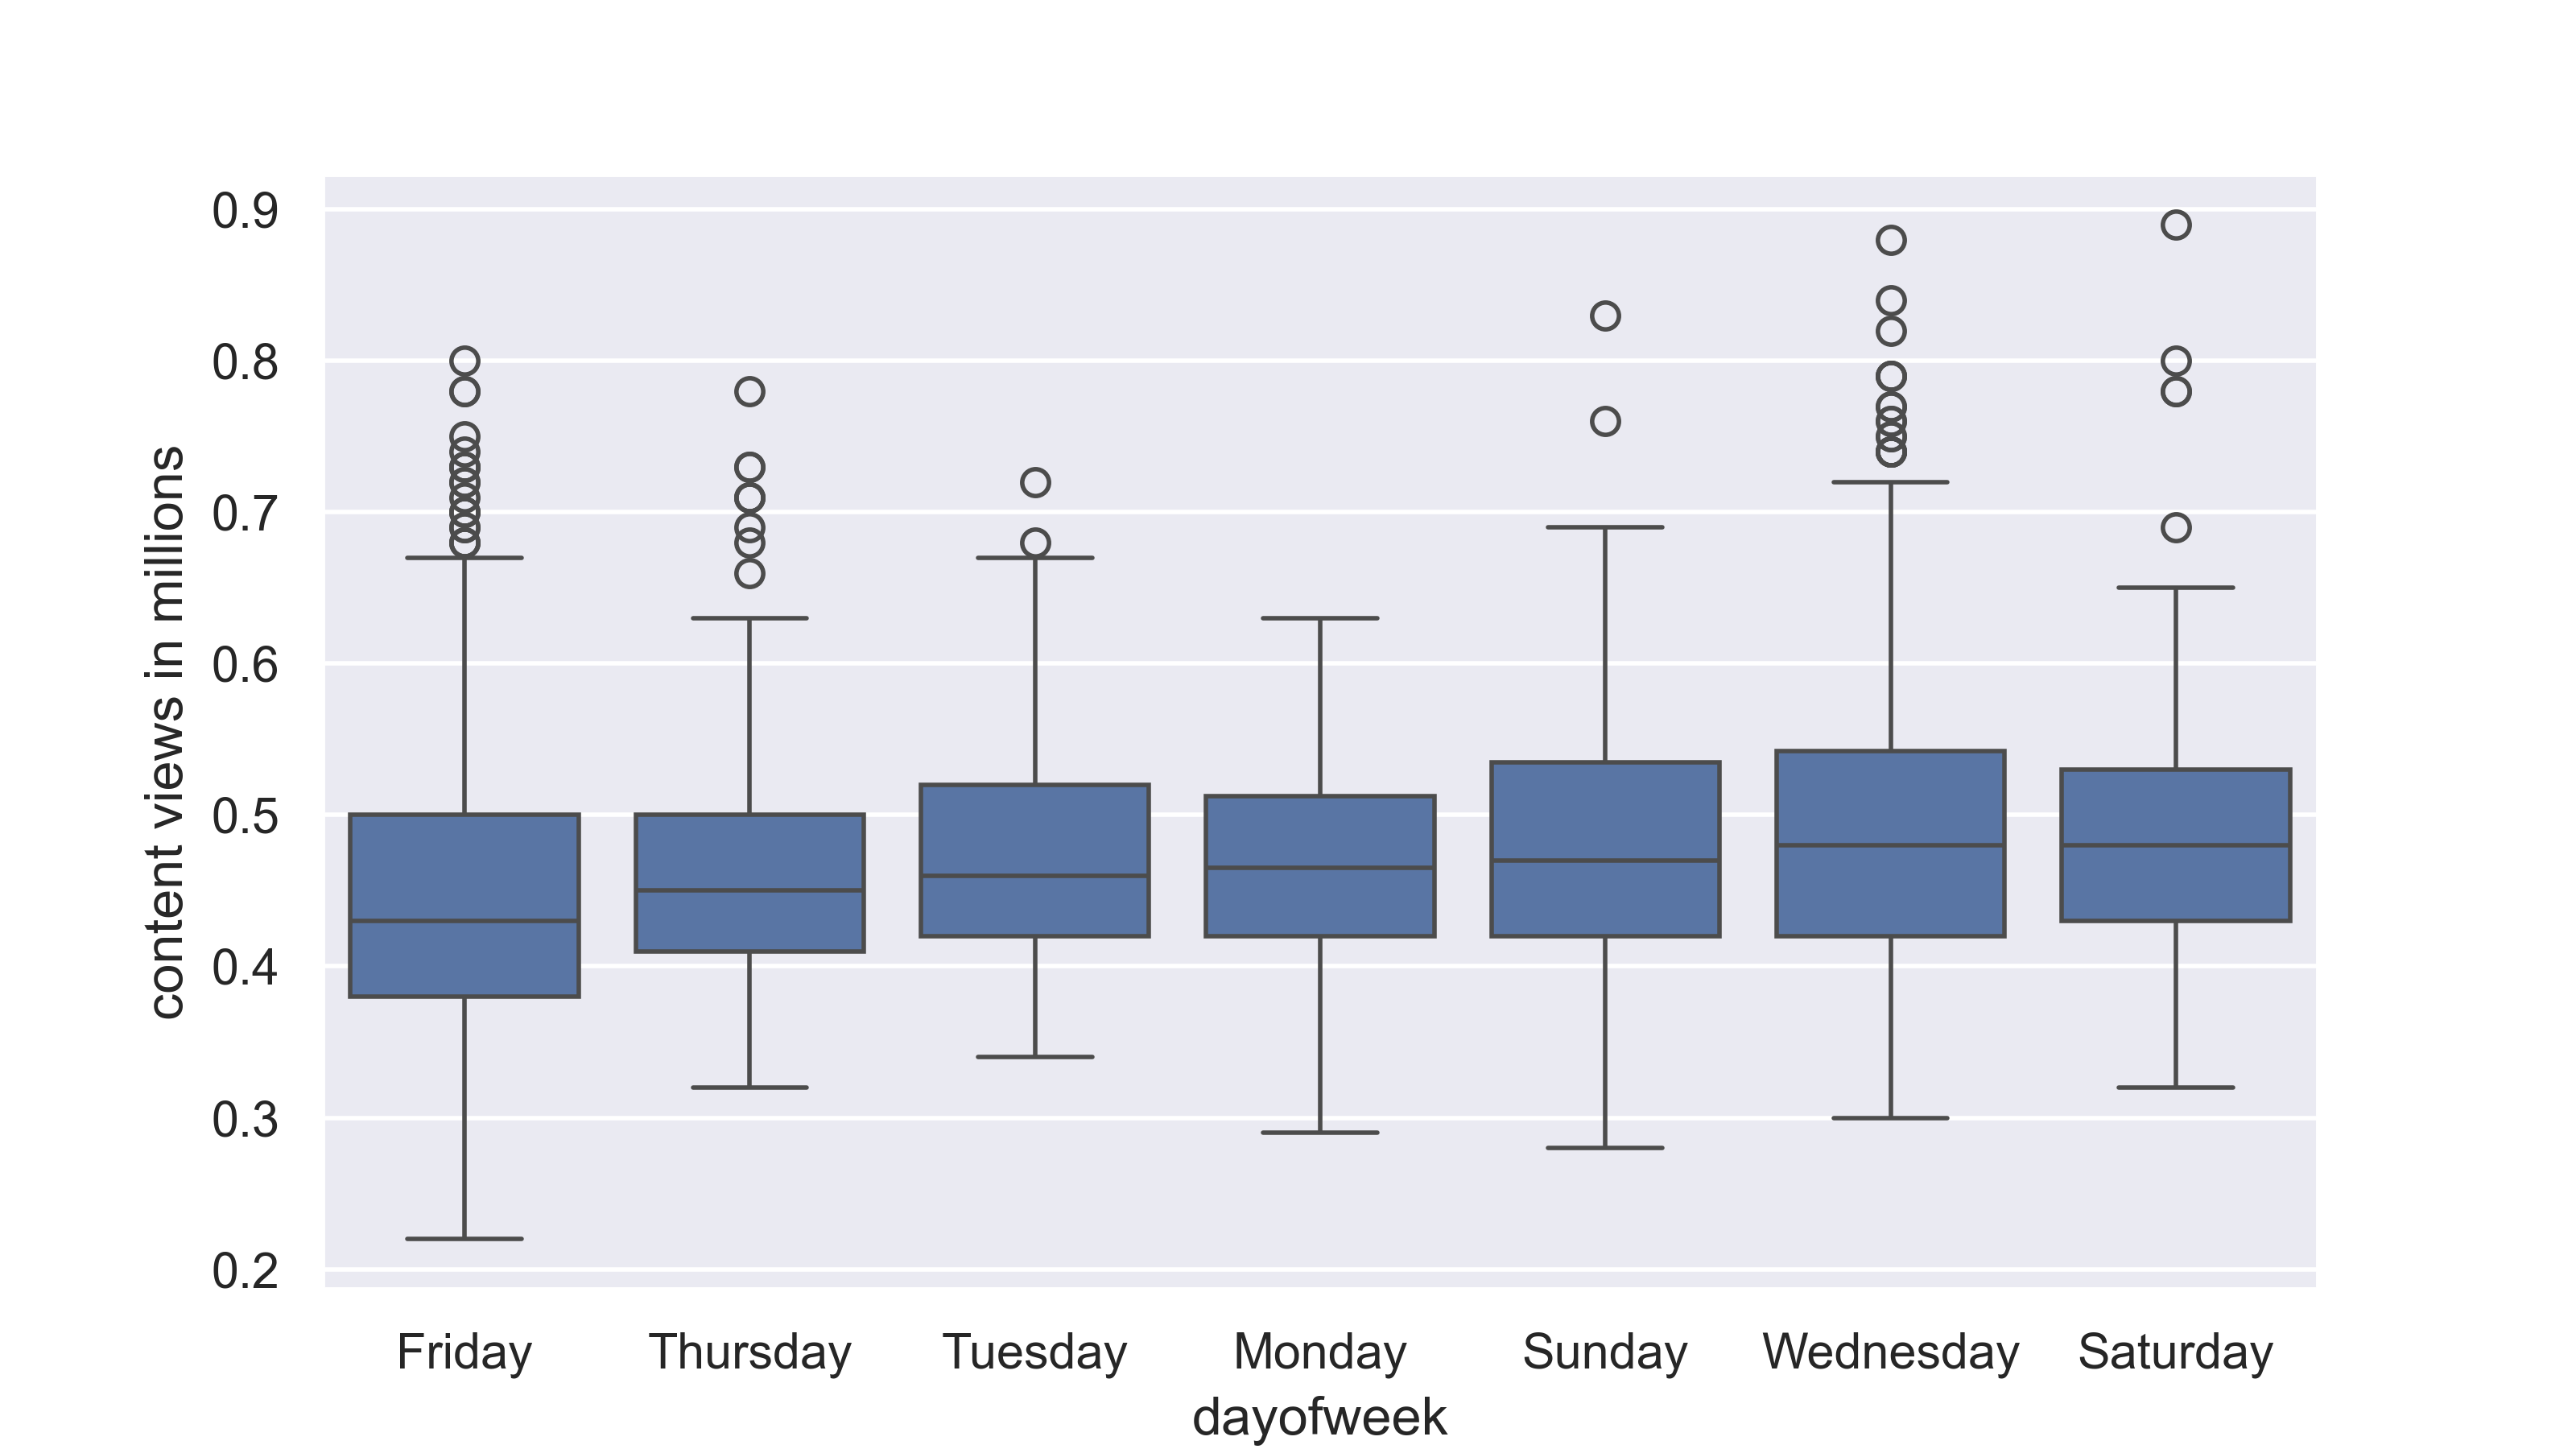
\includegraphics[width=\textwidth]{content_views_vs_dayofweek.png}
		\caption{}
		\label{fig:content_views_vs_dayofweek}
	\end{subfigure}
	\hfill
	\begin{subfigure}[t]{0.49\textwidth}
		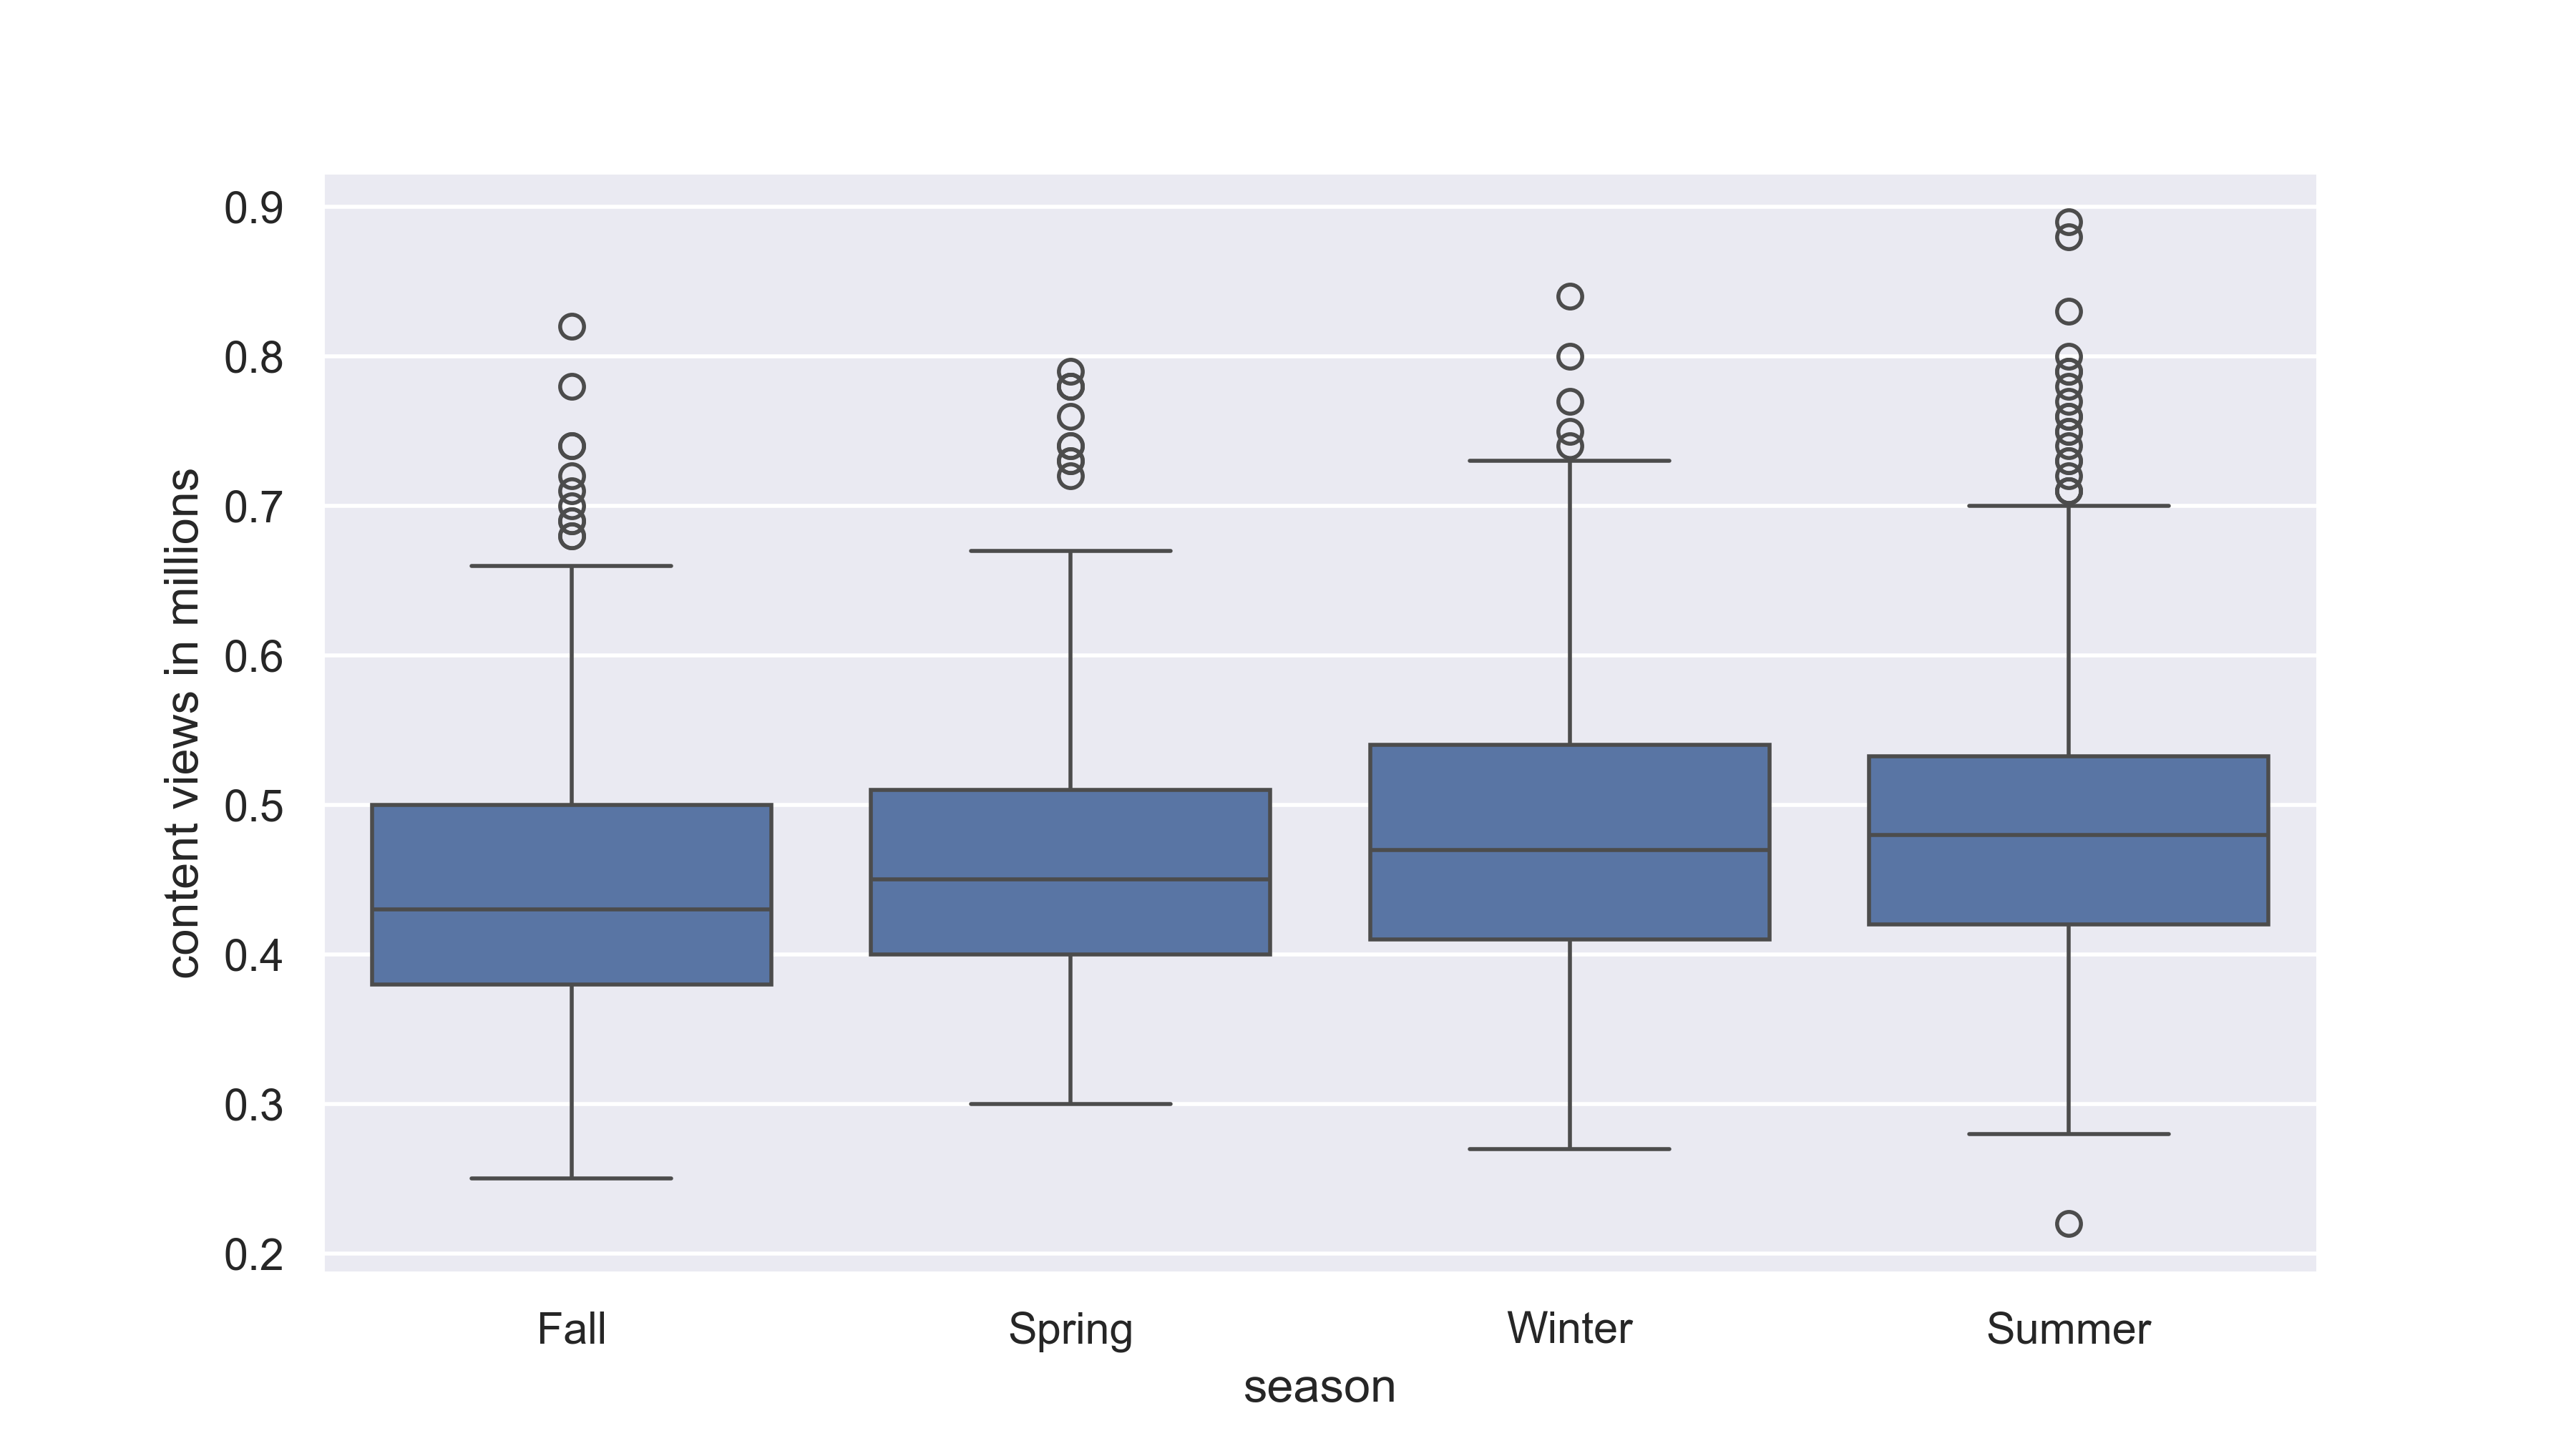
\includegraphics[width=\textwidth]{content_views_vs_season.png}
		\caption{}
		\label{fig:content_views_vs_season}
	\end{subfigure}
	\caption{Effect of day of release and season of release on content view}
	\label{fig:day and season effect}
\end{figure}
It is important also to note that there are other factors in play here. Presence of major sports event on day of show release has strong influence on content views on the first day as shown in figure \ref{fig:Effect of major sports event on content view}. On the left  box plot for content views with respect to presence of major sport event shows that the median value first day viewership get lower. This happens with all kind of genres as shown on right \ref{fig:views_count_sports_event_genre.png}. Also we noticed that in summer there is less number of major sports event as shown in figure \ref{fig:sports_vs_season}. So it could be a interlinked reason for the highest number of views for shows released in summer.      
\begin{figure}[h]
	\centering
	\begin{subfigure}[t]{0.49\textwidth}
		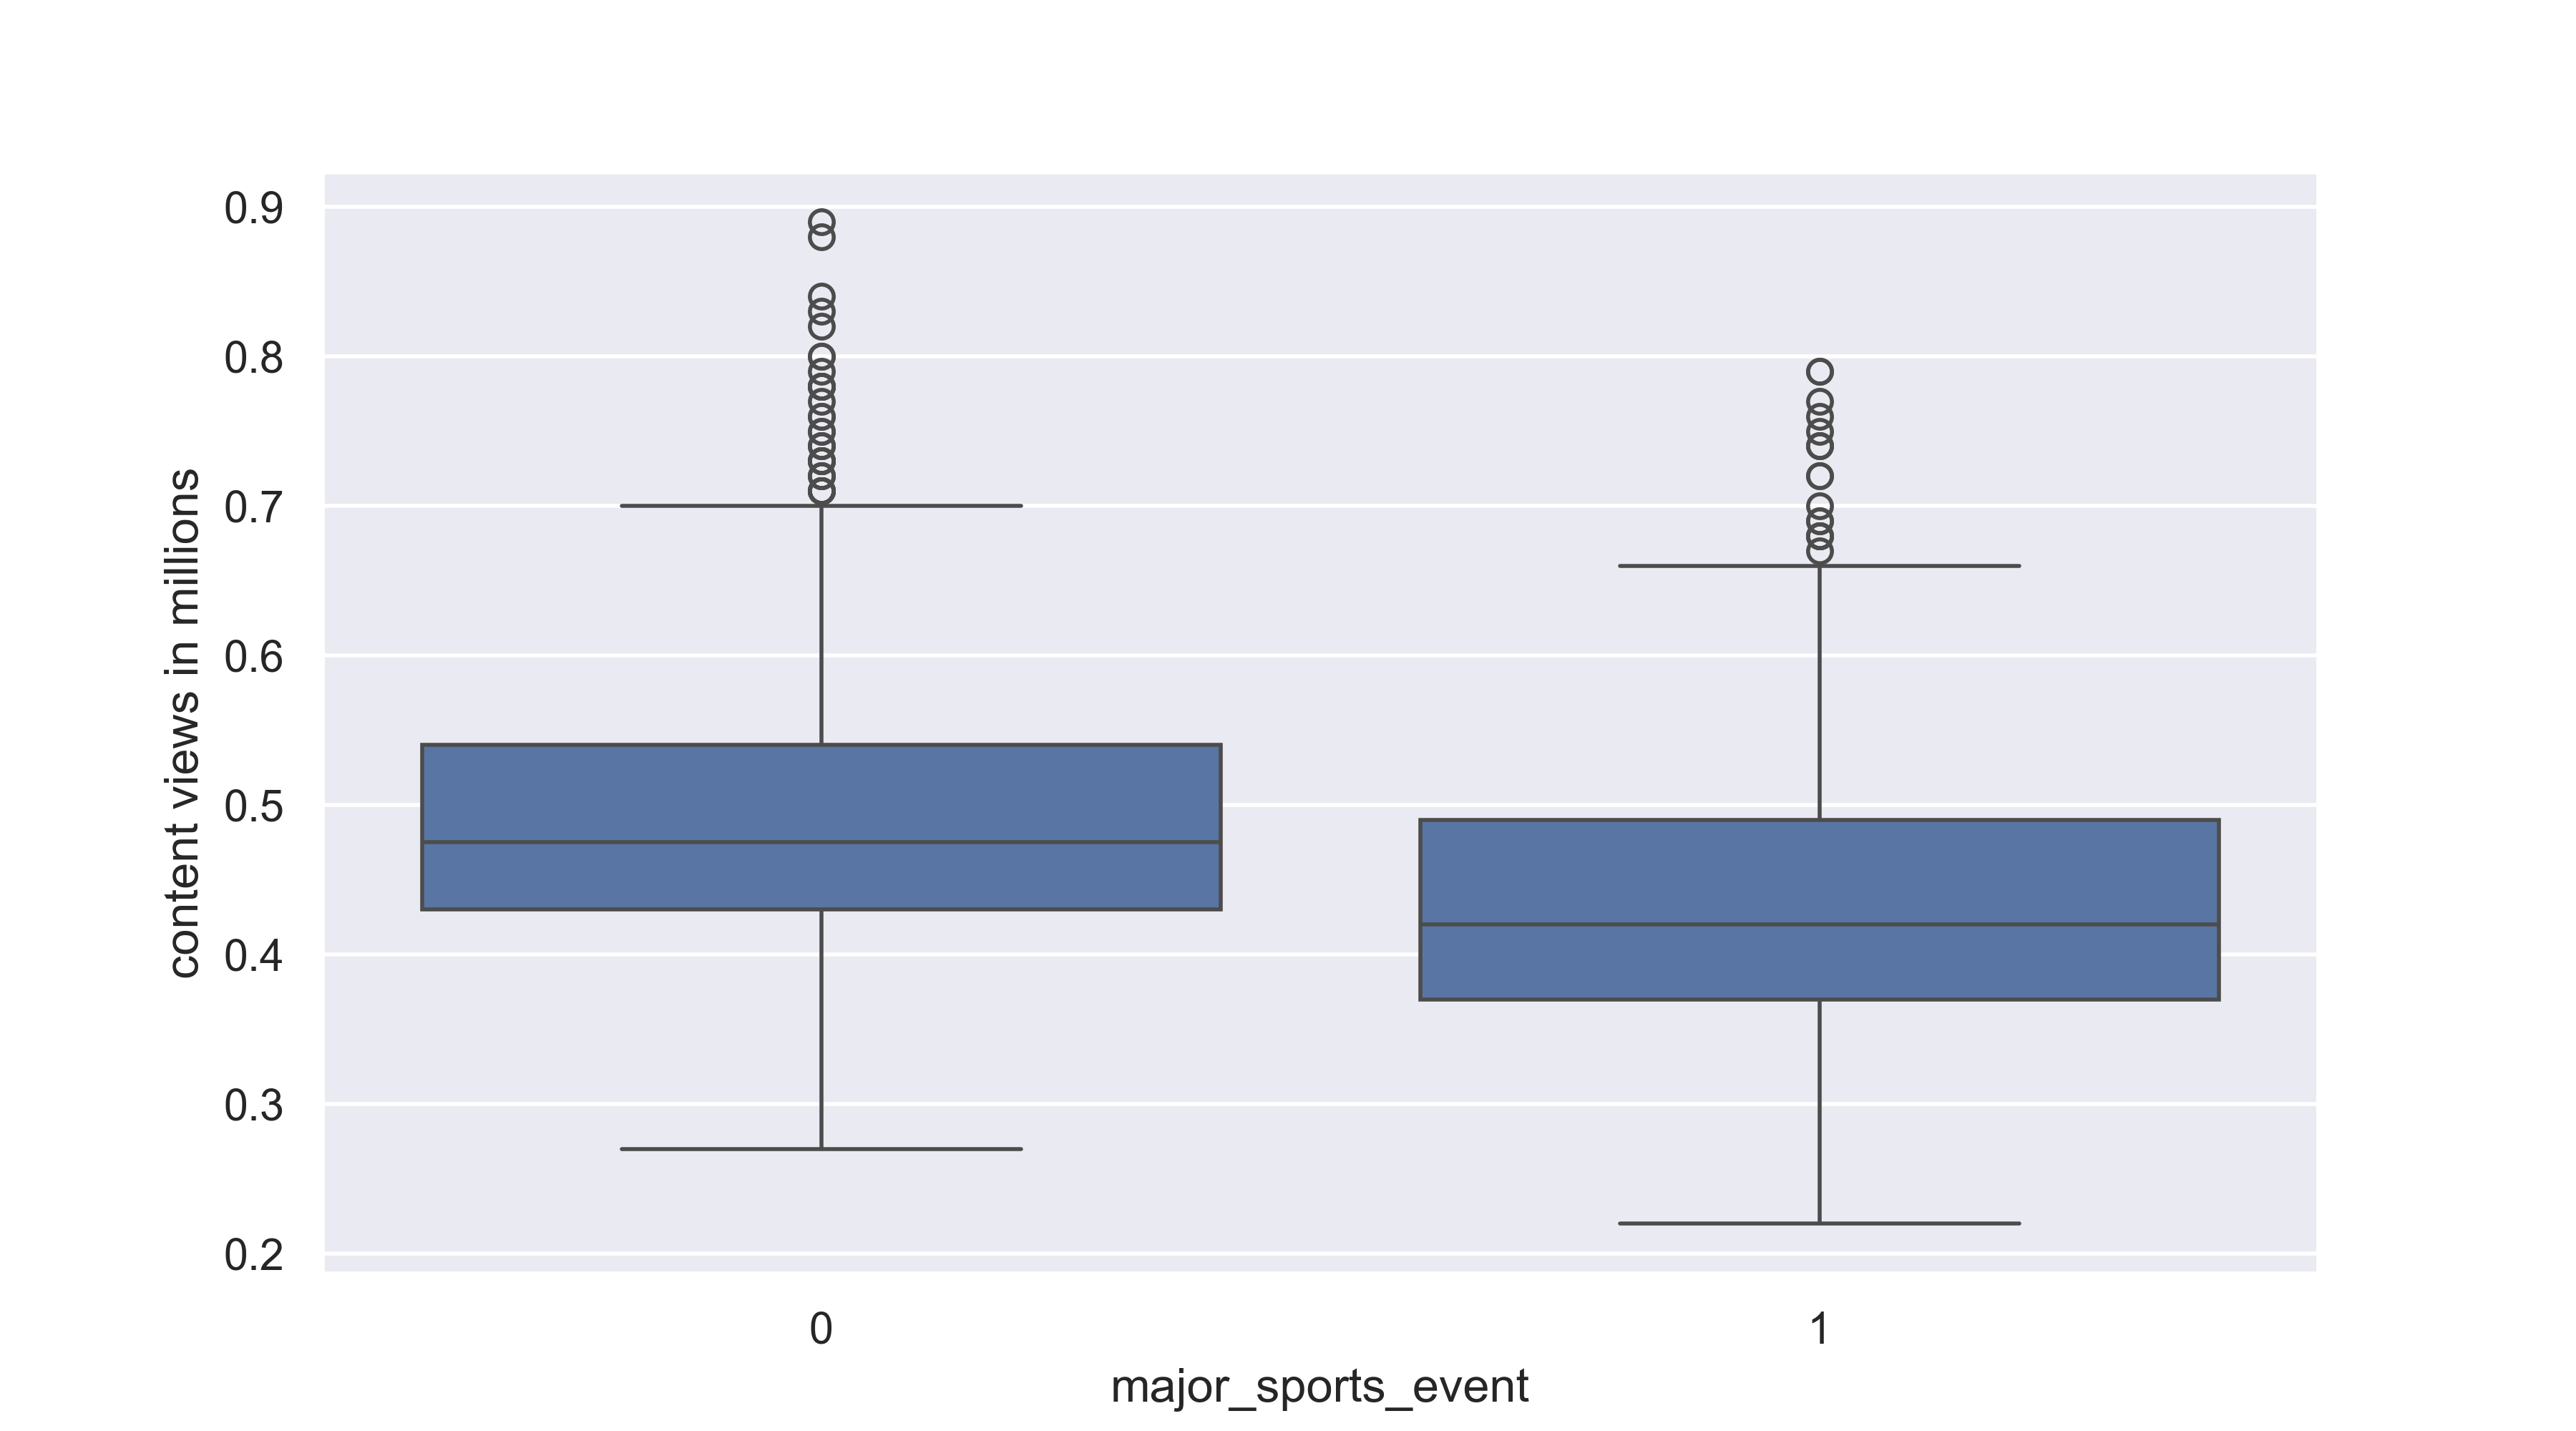
\includegraphics[width=\textwidth]{major_sports_event_vs_content_views.png}
		\caption{content views box plot with respect to major sports event}
		\label{fig:major_sports_event_vs_content_views.png}
	\end{subfigure}
	\hfill
	\begin{subfigure}[t]{0.49\textwidth}
		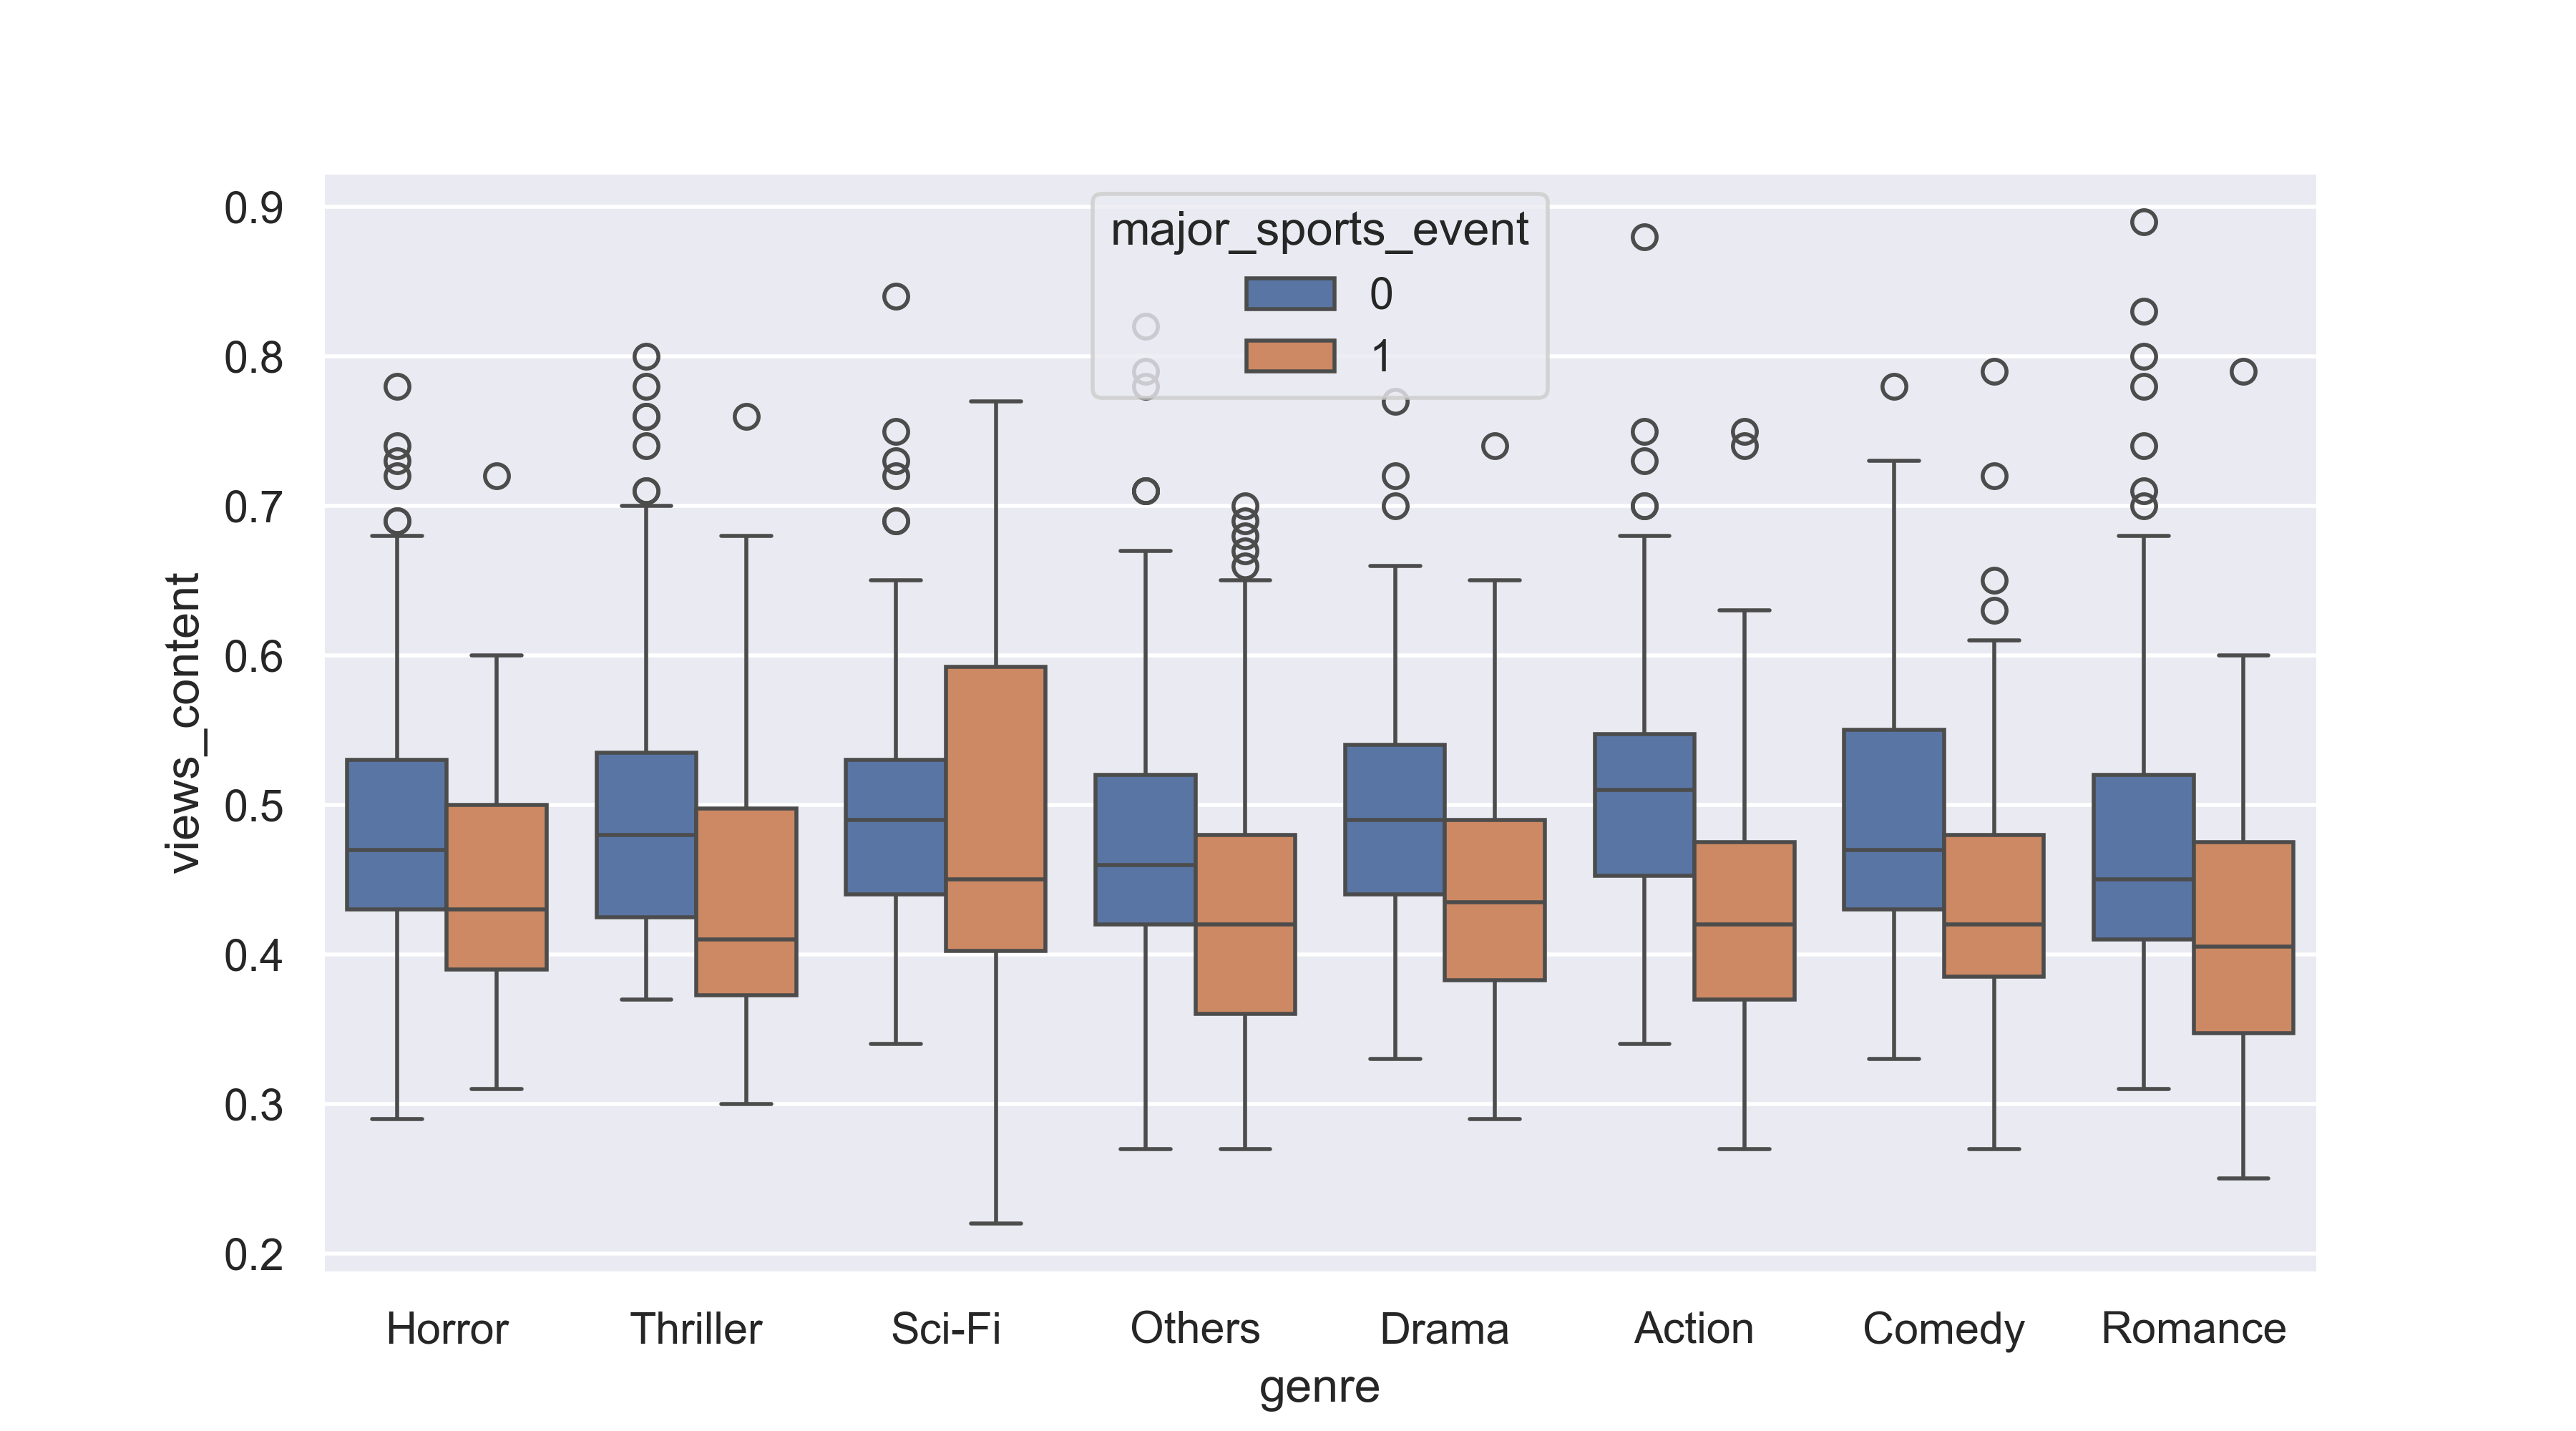
\includegraphics[width=\textwidth]{views_count_sports_event_genre.png}
		\caption{content views box plot with respect to major sports event as well as all genres.}
		\label{fig:views_count_sports_event_genre.png}
	\end{subfigure}
		\hfill
	\begin{subfigure}[t]{0.49\textwidth}
		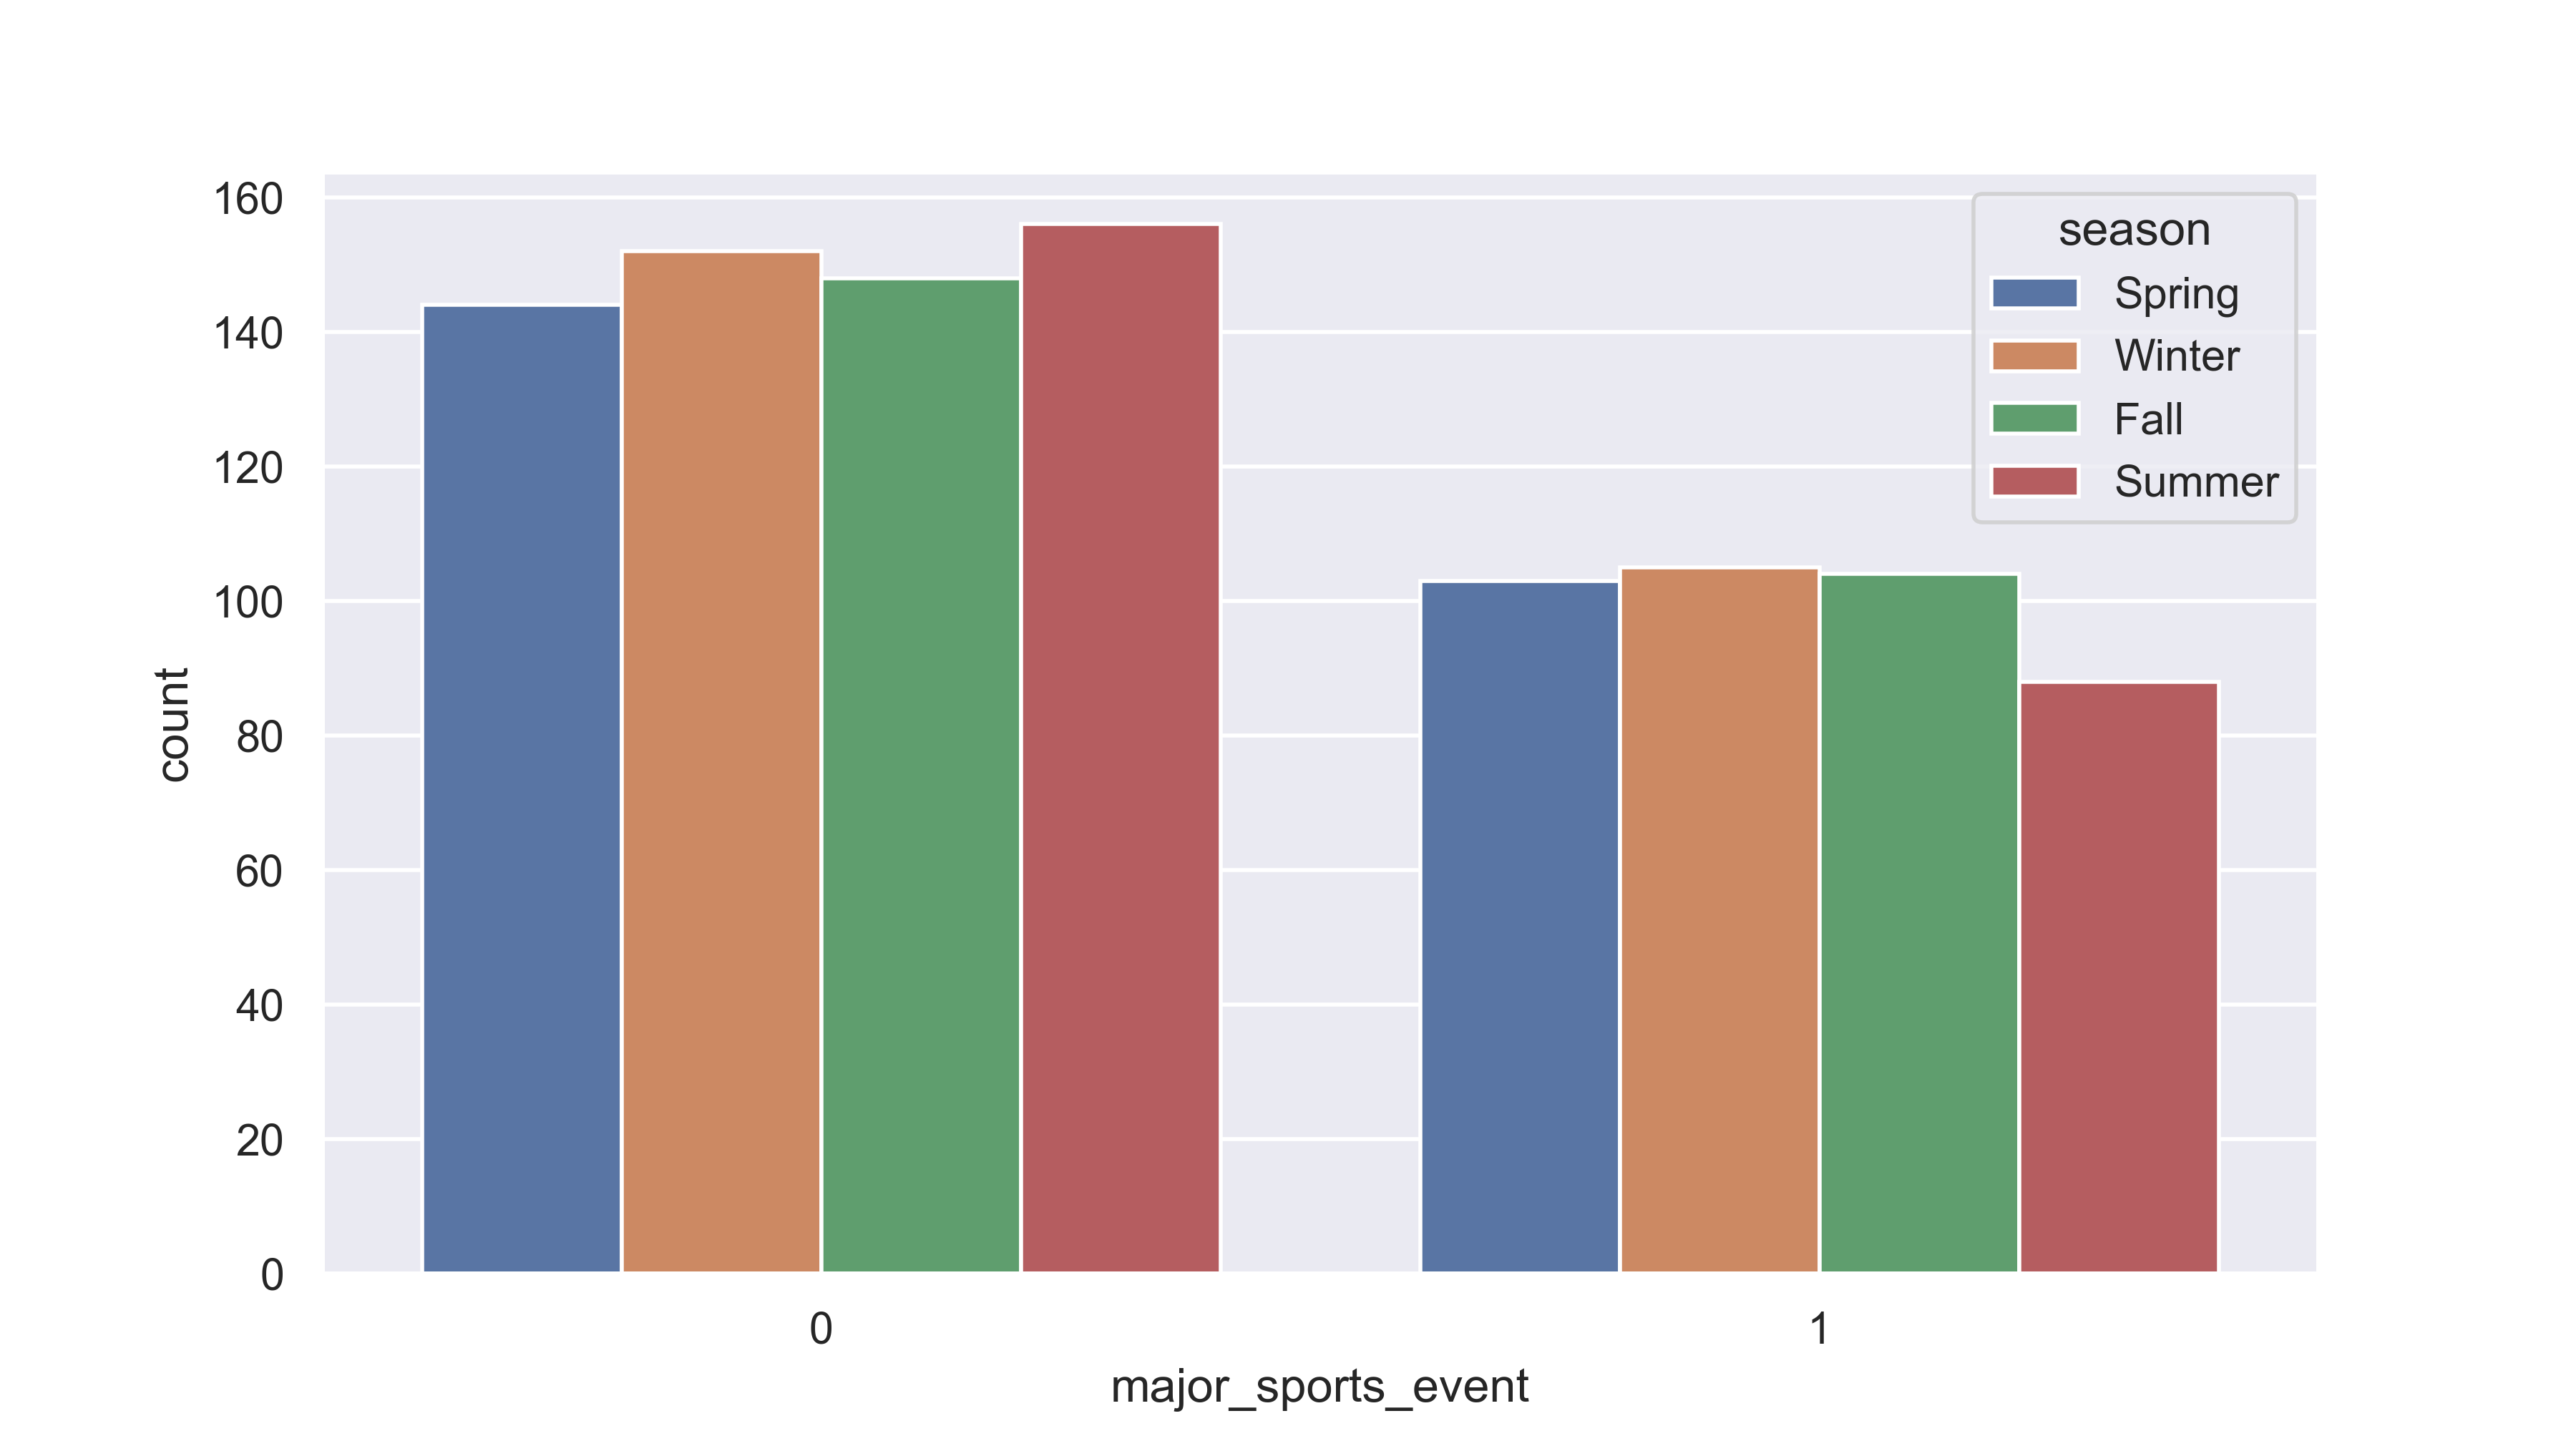
\includegraphics[width=\textwidth]{sports_vs_season.png}
		\caption{In summer there is lesser clash with major sports event as seen on the second column of the bar plot.}
		\label{fig:sports_vs_season}
	\end{subfigure}
	\caption{Effect of major sports event on content view}
	\label{fig:Effect of major sports event on content view}
\end{figure}
\subsection{What is the correlation between trailer views and content views?}
As shown in Figure \ref{fig:corr} we have plotted the correlation among all the numerical variables. We observe that there is a weak correlation of 0.26 between number visitors to the platform on previous week and content views and a strong correlation of 0.75 between trailer views and content views. To further illustrate we have shown a scatter plot between them on figure \ref{fig:content_vs_trailer}. This gives a strong impression for linear relationship between trailer views and content views. We observe that there is practically very weak correlation among predictor variables. This is a good sign when we will consider building linear model in the coming section. One more important point note here is that the correlation between ad impressions and content views is very weak 0.05. This hints us towards lack of effectiveness in the ad campaigns in influencing customers for the up coming shows. For a successful ad campaign we would want a strong positive correlation.
\begin{figure}[h]
	\centering
	\begin{subfigure}[t]{0.6\textwidth}
		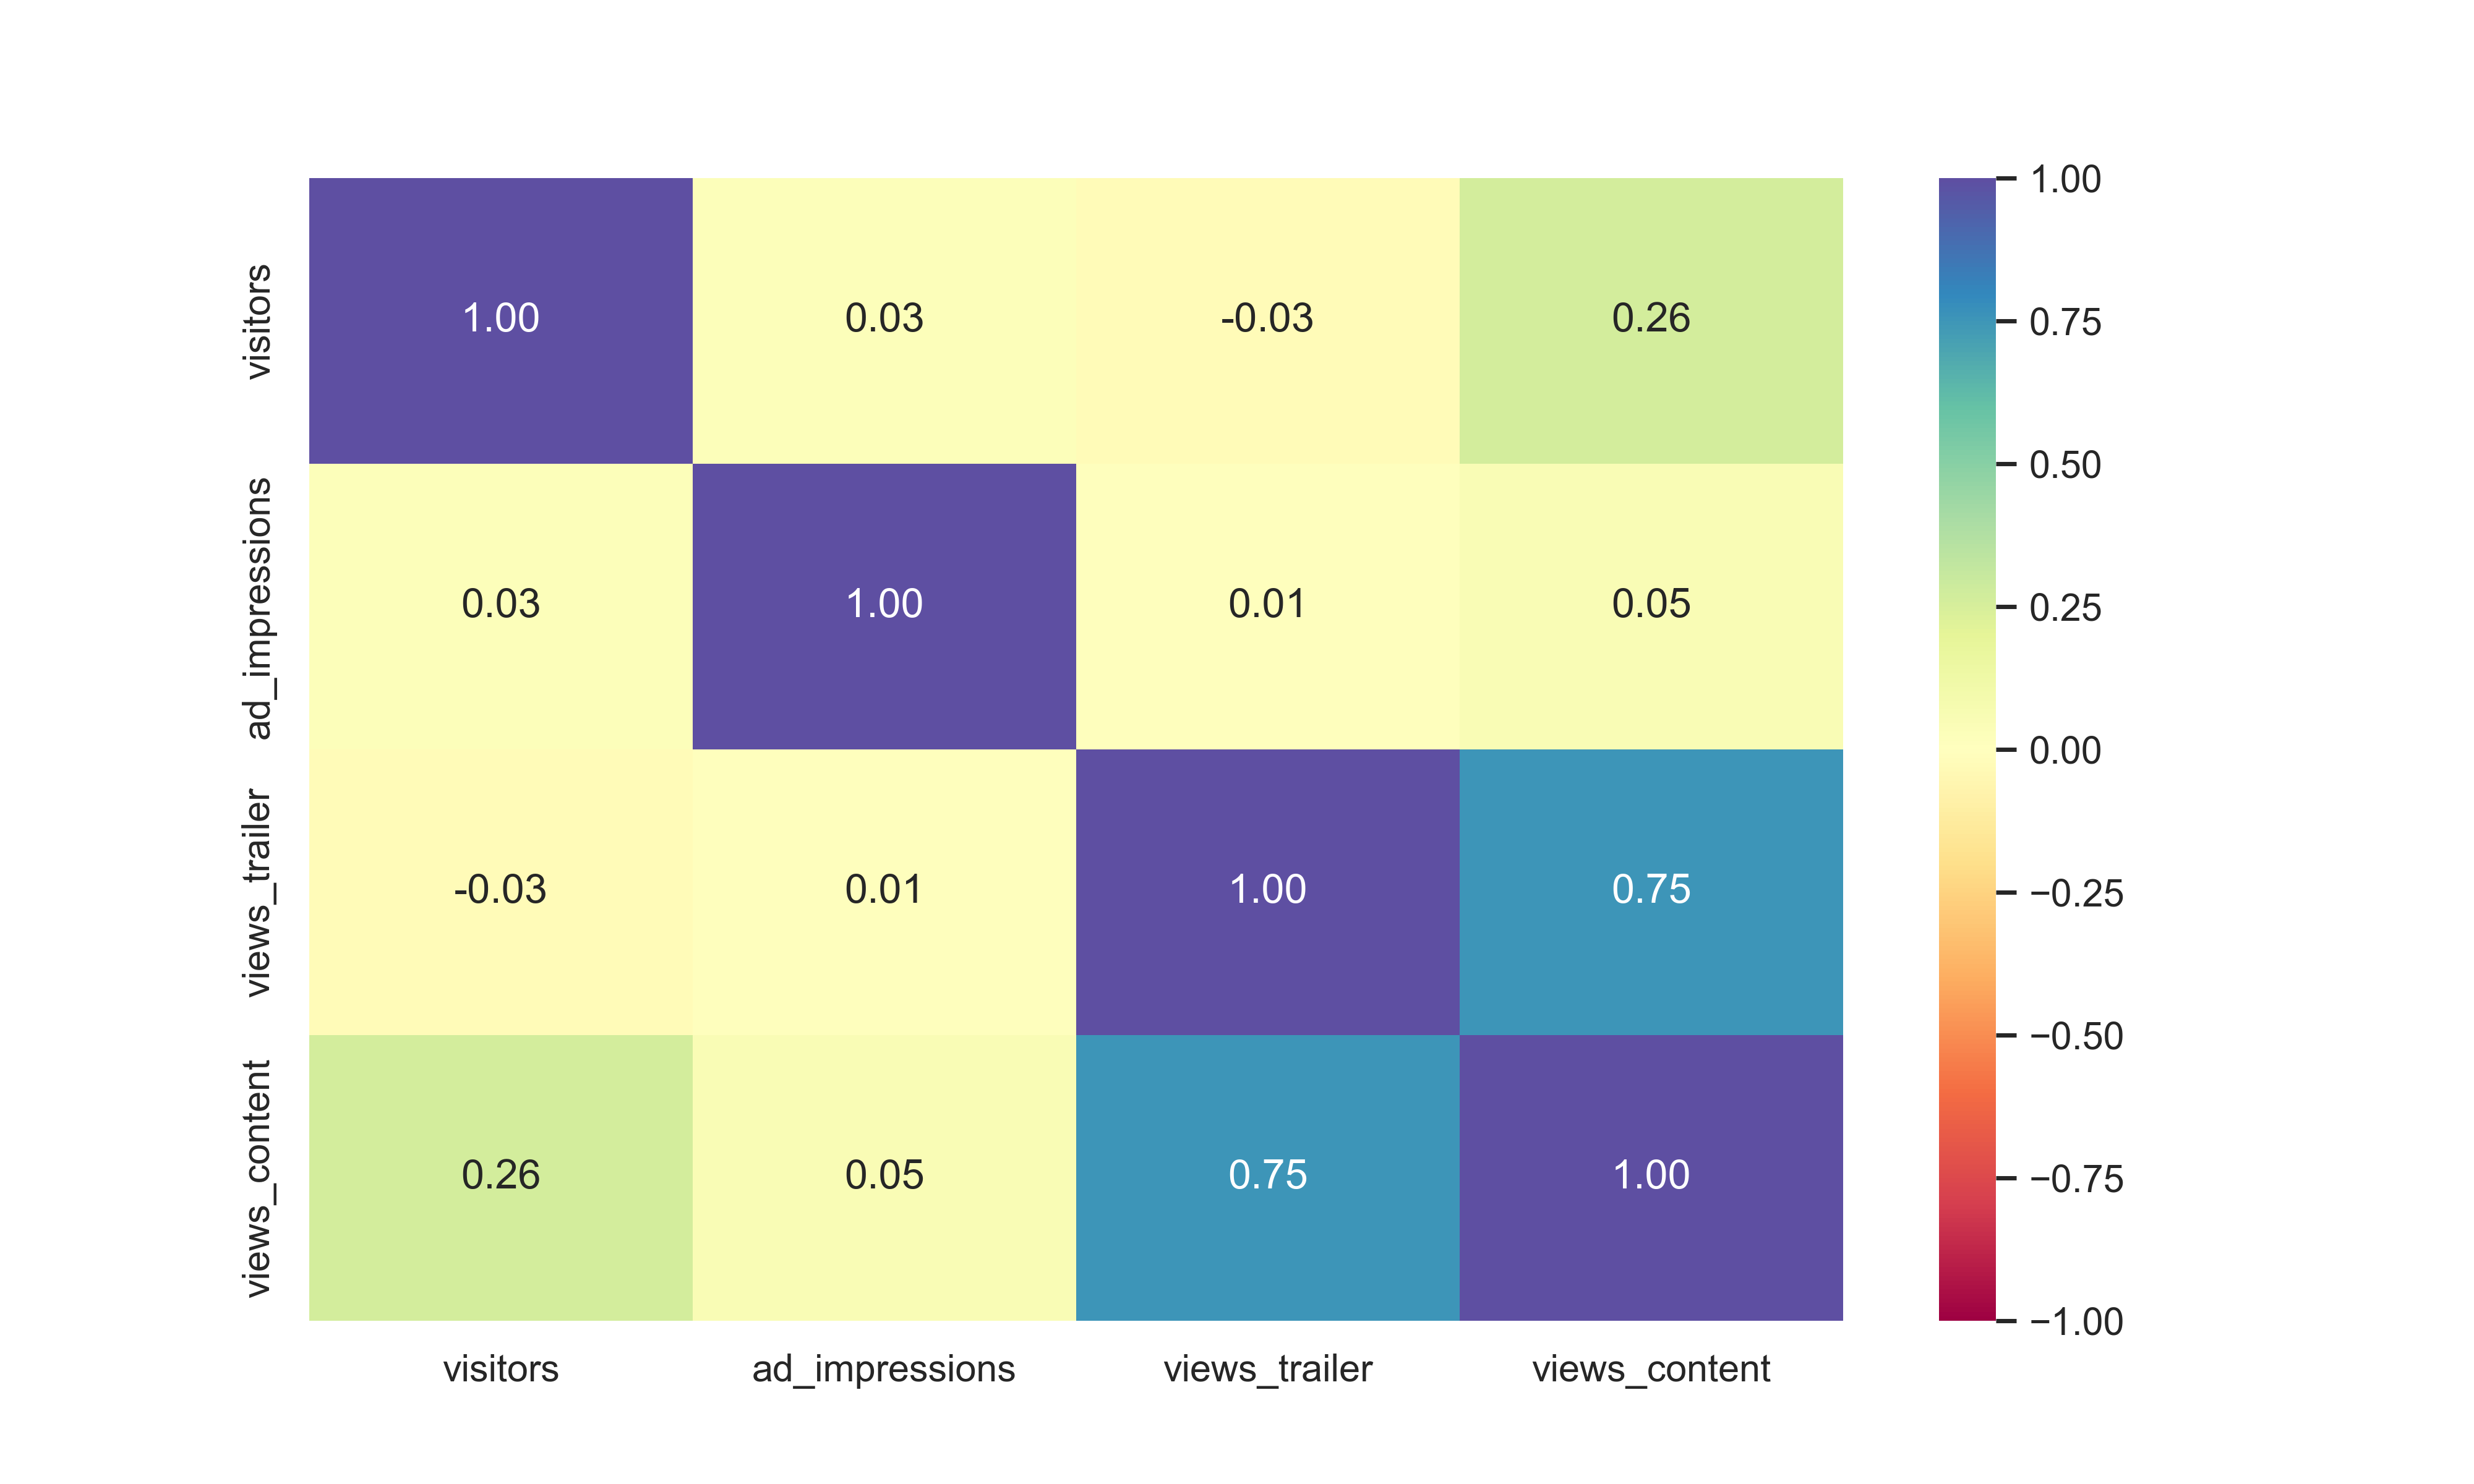
\includegraphics[width=\textwidth]{corr.png}
		\caption{Correlation among numerical variables}
		\label{fig:corr}
	\end{subfigure}
	\hfill
	\begin{subfigure}[t]{0.39\textwidth}
		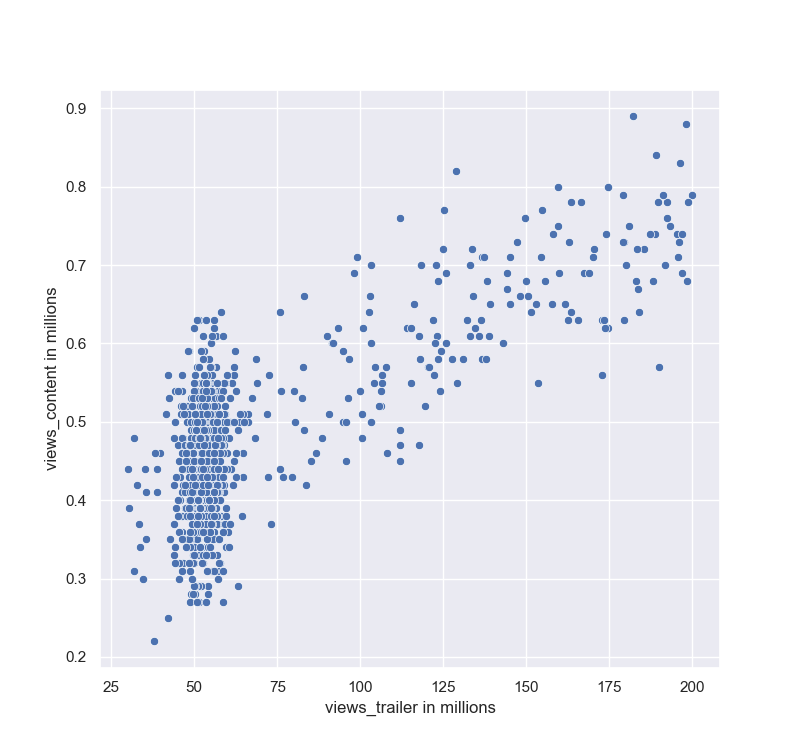
\includegraphics[width=\textwidth]{content_vs_trailer.png}
		\caption{Scatter plot of content views vs trailer views.}
		\label{fig:content_vs_trailer}
	\end{subfigure}
	\caption{Correlation plot}
	\label{fig:correlation}
\end{figure}
\section{Linear Regression model}
In this section we will describe the implementation of Linear regression model on our content views data set. As we had already seen in the figure \ref{fig:content_vs_trailer} there is a graphical impression of linear dependence between content views and trailer views. Being the simplest and most popular model we will implement it with respect to all independent variables. Here our target variable is content views and all other variables are independent/predictor variables. We will proceed with assumption that linear dependency is a good description of target variable in terms of predictor variables. More precisely our model equation has following form:
\begin{equation}
	\hat{y}=\sum_i \beta_i.X_i + C 
\end{equation}
Where $\hat{y}$ is the target variable we want to predict. $X_i$ are predictor/independent variables with $\beta_i$ as coefficients. C is the intercept which is the value of target variable when all independent variables are zero. epsilon is the noise or error term  So we are expressing target variable as a linear combination of independent variables. We used ordinary least square method for the regression. Mean while it is important to note that here calculating $\beta_i$s from sample data are an estimation of population parameter/coefficients. We assume that the data are drawn from population in following manner:
\begin{equation}
	\hat{y}=\sum_i \beta^{pop}_i.X_i + C^{pop} + \epsilon 
\end{equation}
where $\epsilon$ is the error or noise term which is assumed to normally distributed. Therefore the calculation of $\beta_i$ from sample data is the estimation of population coefficients $\beta^{pop}_i$. The assumptions of linear regression are listed below.
\begin{enumerate}
	\item We assume there is a linear relationship between target and independent variable. More precisely the data are drawn from population according to equation 2 and expectation value of error term i.e $E(\epsilon)$ = 0 and $E(y)$ = $\sum_i \beta^{pop}_i.X_i + C^{pop}$.
	\item The error terms are independent for each target variable value.
	\item The error terms are normally distributed.
	\item Homoscedasticity: The error terms have equal variance for each target variable.
	\item There is no strong multicollinearity among independent variables.
\end{enumerate}
	\begin{wrapfigure}{R}{0.25\textwidth}
	%\vspace{-1mm} % move picture up
	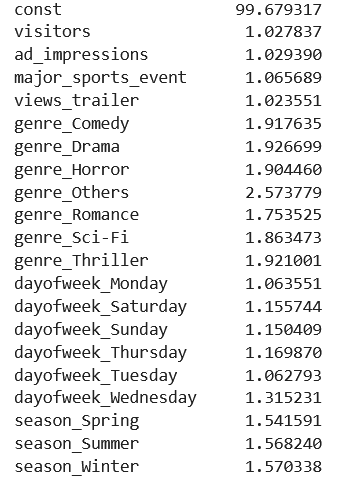
\includegraphics[width=0.25\textwidth]{VIF.png}
	\vspace{-4mm} % spacing between figure and caption
	\caption{\small{Variance inflation factor for all predictors}}
	\label{fig:VIF}
	\end{wrapfigure}
	In a sentence we can say about the assumptions as : error terms $\epsilon$ are independent Normal random variable with mean zero and constant variance. During model implementation we check for validity of all these assumptions. We now describe one of the most important step in predictive modeling which is features preparation or feature engineering. As we have categorical values in our data set we can not use them directly in the regression which requires numerical variables. So we convert them to numerical values by creating dummy variable for each categorical variable with number of new variables being one less than number of unique categories. So these dummy variables have now a value of 1 or 0 corresponding to true or false value for that category value. We divide the data set into 70:30 ratio subsets for training and testing respectively. So out of 1000 data records we use 700 for training and 300 for testing and the sampling is done randomly.  
	On our first trial we tried the model using all the independent variables. On the result we got a R-squared value of 0.7916 and root mean squared error(RMSE) value of 0.0485. $R^2$ is a measure of how strong is the linear relationship. So 79.16 \% of variance in the target variable is explained by this model in terms of predictor variables. To ensure that there is no multicollinearity among predictors we checked the variance inflation factor VIF for each variable. Figure \ref{fig:VIF} shows the list of VIF for all variables. As a generally followed rule If VIF is 1, then there is no correlation among the $k^{th}$ predictor and the remaining predictor variables, and hence, the variance of $\beta_k$ is not inflated at all. If VIF exceeds 5, we say there is moderate VIF, and if it is 10 or exceeding 10, it shows signs of high multi-collinearity. Ignoring the intercept which is a constant all other variables have VIF less than 5. Therefore our model does not have multicollinearity. Hereby we have validated the assumption corresponding to multicollinearity. 
	
	The p values in the fit result ($P > |t|$) are interpreted in the following ways.	
		For each predictor variable there is a null hypothesis and alternate hypothesis.
			Null hypothesis : Predictor variable is not significant
			Alternate hypothesis : Predictor variable is significant
		($P > |t|$) gives the p-value for each predictor variable to check the null hypothesis.
		If the level of significance is set to 5\% (0.05), the p-values greater than 0.05 would indicate that the corresponding predictor variables are not significant.
	We found the p values for ad impressions, and genre variables and day of week Tuesday variable significantly higher than 0.05. Therefore we have removed these predictors from our final linear model. The coefficients from fit results of final model are shown in figure \ref{fig:coeff}. The model performance on the training and test data set is shown in figure \ref{fig:final model performance}. To test the independence of residuals or error terms we have shown fitted vs residual plot on figure \ref{fig:Fitted_Vs_Residual}. The random scattering of residual around x axis shows that our assumption on Linearity dependence of target variable and independence of residuals are valid. To test the normality of error term we have plotted distribution of residuals on figure \ref{fig: normality check} and a Q-Q plot which is a comparison of quantile by quantile with respect to the normal distribution. The distribution of residuals closely look like a normal distribution but with a longer right tail. The deviation on both tails are visible on the Q-Q plot.  
\begin{figure}[h]
	%\vspace{-1mm} % move picture up
	\centering
	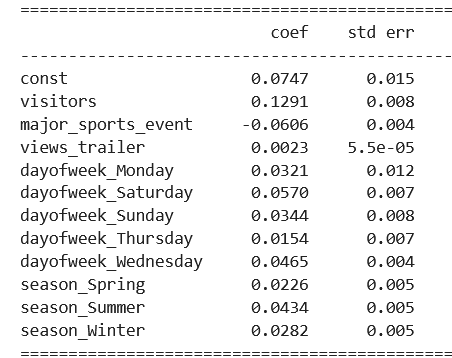
\includegraphics[width=0.5\textwidth]{final_coeff.png}
	\caption{\small{Coefficients with standard error from fit result of final model.}}
	\label{fig:coeff}
\end{figure}
\begin{figure}[h]
	\centering
	\begin{subfigure}[t]{0.45\textwidth}
		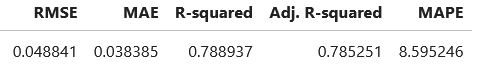
\includegraphics[width=\textwidth]{training_performance.png}
		\caption{}
		\label{fig:}
	\end{subfigure}
	\hfill
	\begin{subfigure}[t]{0.45\textwidth}
		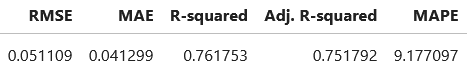
\includegraphics[width=\textwidth]{test_performance.png}
		\caption{}
		\label{fig:}
	\end{subfigure}
	\caption{Model performance on training and test data.}
	\label{fig:final model performance}
\end{figure}
We also carried out Shapiro-Wilk test for testing the validity of normality. We got a p value of 0.3 which is not sufficient to reject the null hypothesis that distribution is normal. Hence our assumption of normality is valid. For the test of constant variance we carried out the Goldfeld–Quandt test which checks for heteroscedasticity in regression analyses. We got a p value of 0.128 hence we can not reject the null hypothesis that variances are equal. So all of the 5 assumptions are valid in our model for practical purpose. As we see from figure \ref{fig:final model performance}, we can see that RMSE on the train and test sets are comparable. So, our model is not suffering from overfitting. R-squared of the model is 0.761 and adjusted R-squared is 0.751, which shows that the model is able to explain ~75\% variance in the data. The MAPE on the test set suggests we can predict within 9.17\% of the content views. This can be considered a good model. This suggests that the model is effective for both prediction and inference.  	
\begin{figure}[h]
	\centering
	\begin{subfigure}[t]{0.45\textwidth}
		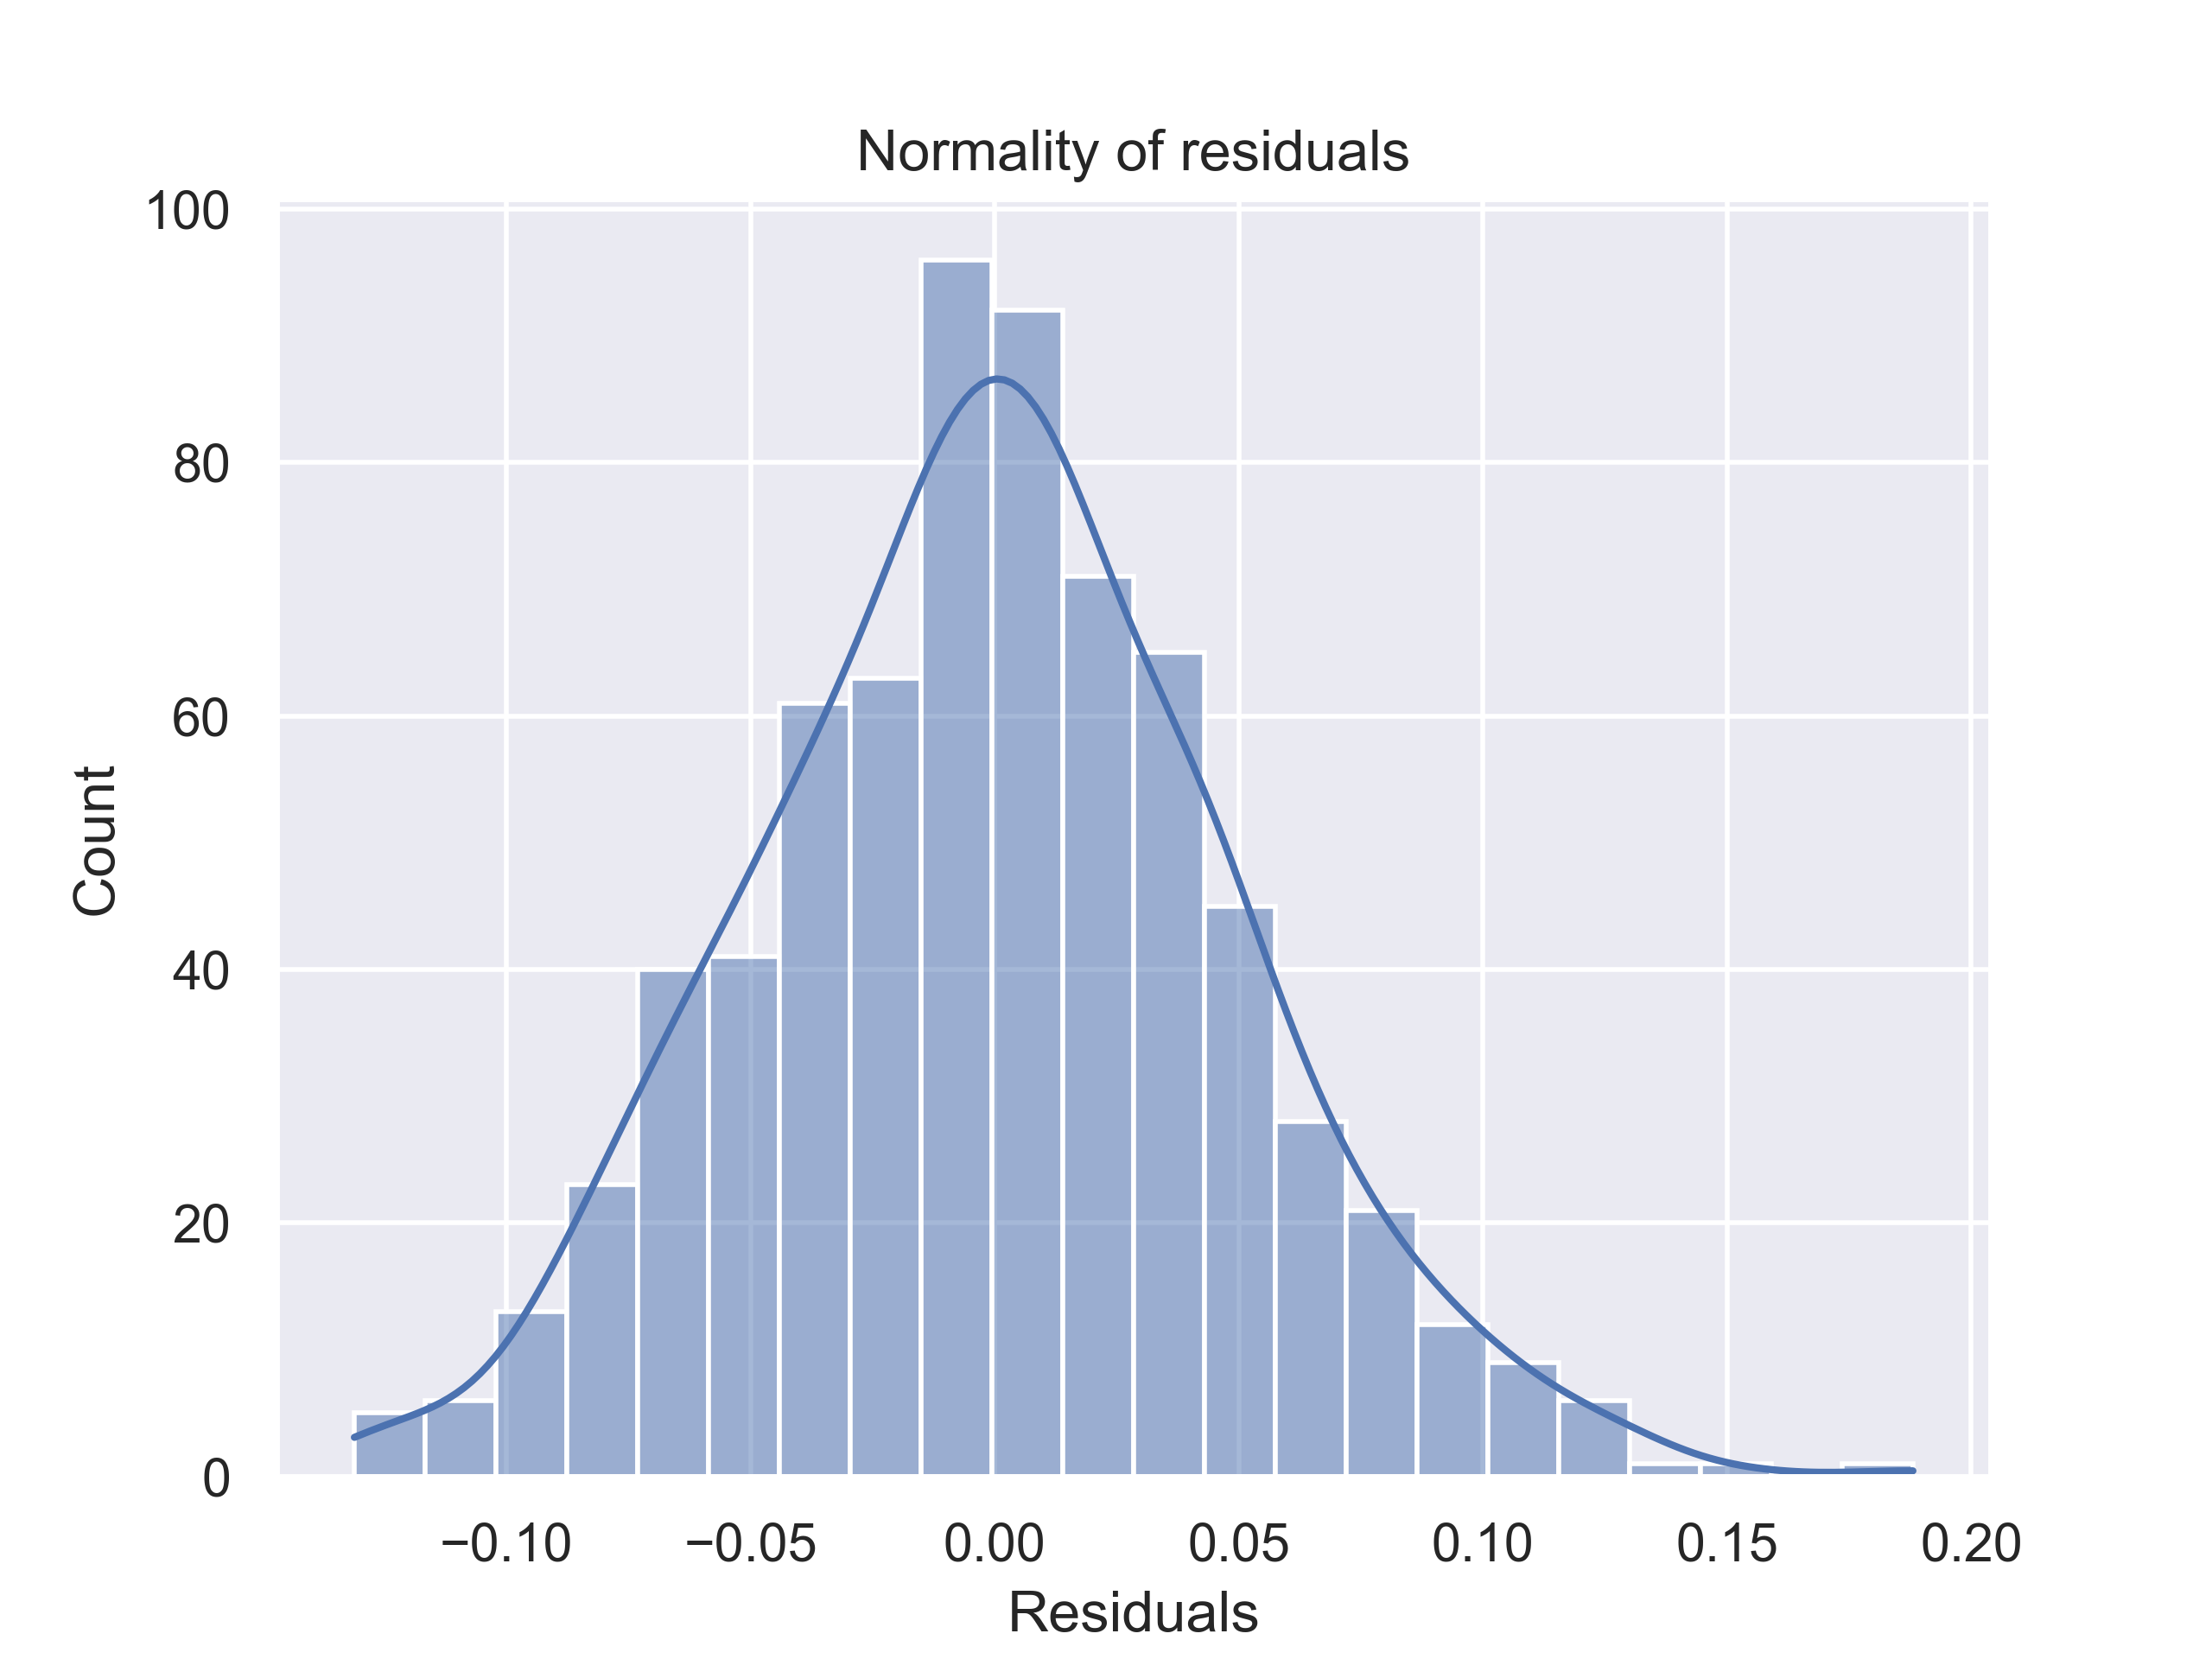
\includegraphics[width=\textwidth]{normality_residuals.png}
		\caption{Distribution of residuals}
		\label{fig:}
	\end{subfigure}
	\hfill
	\begin{subfigure}[t]{0.45\textwidth}
		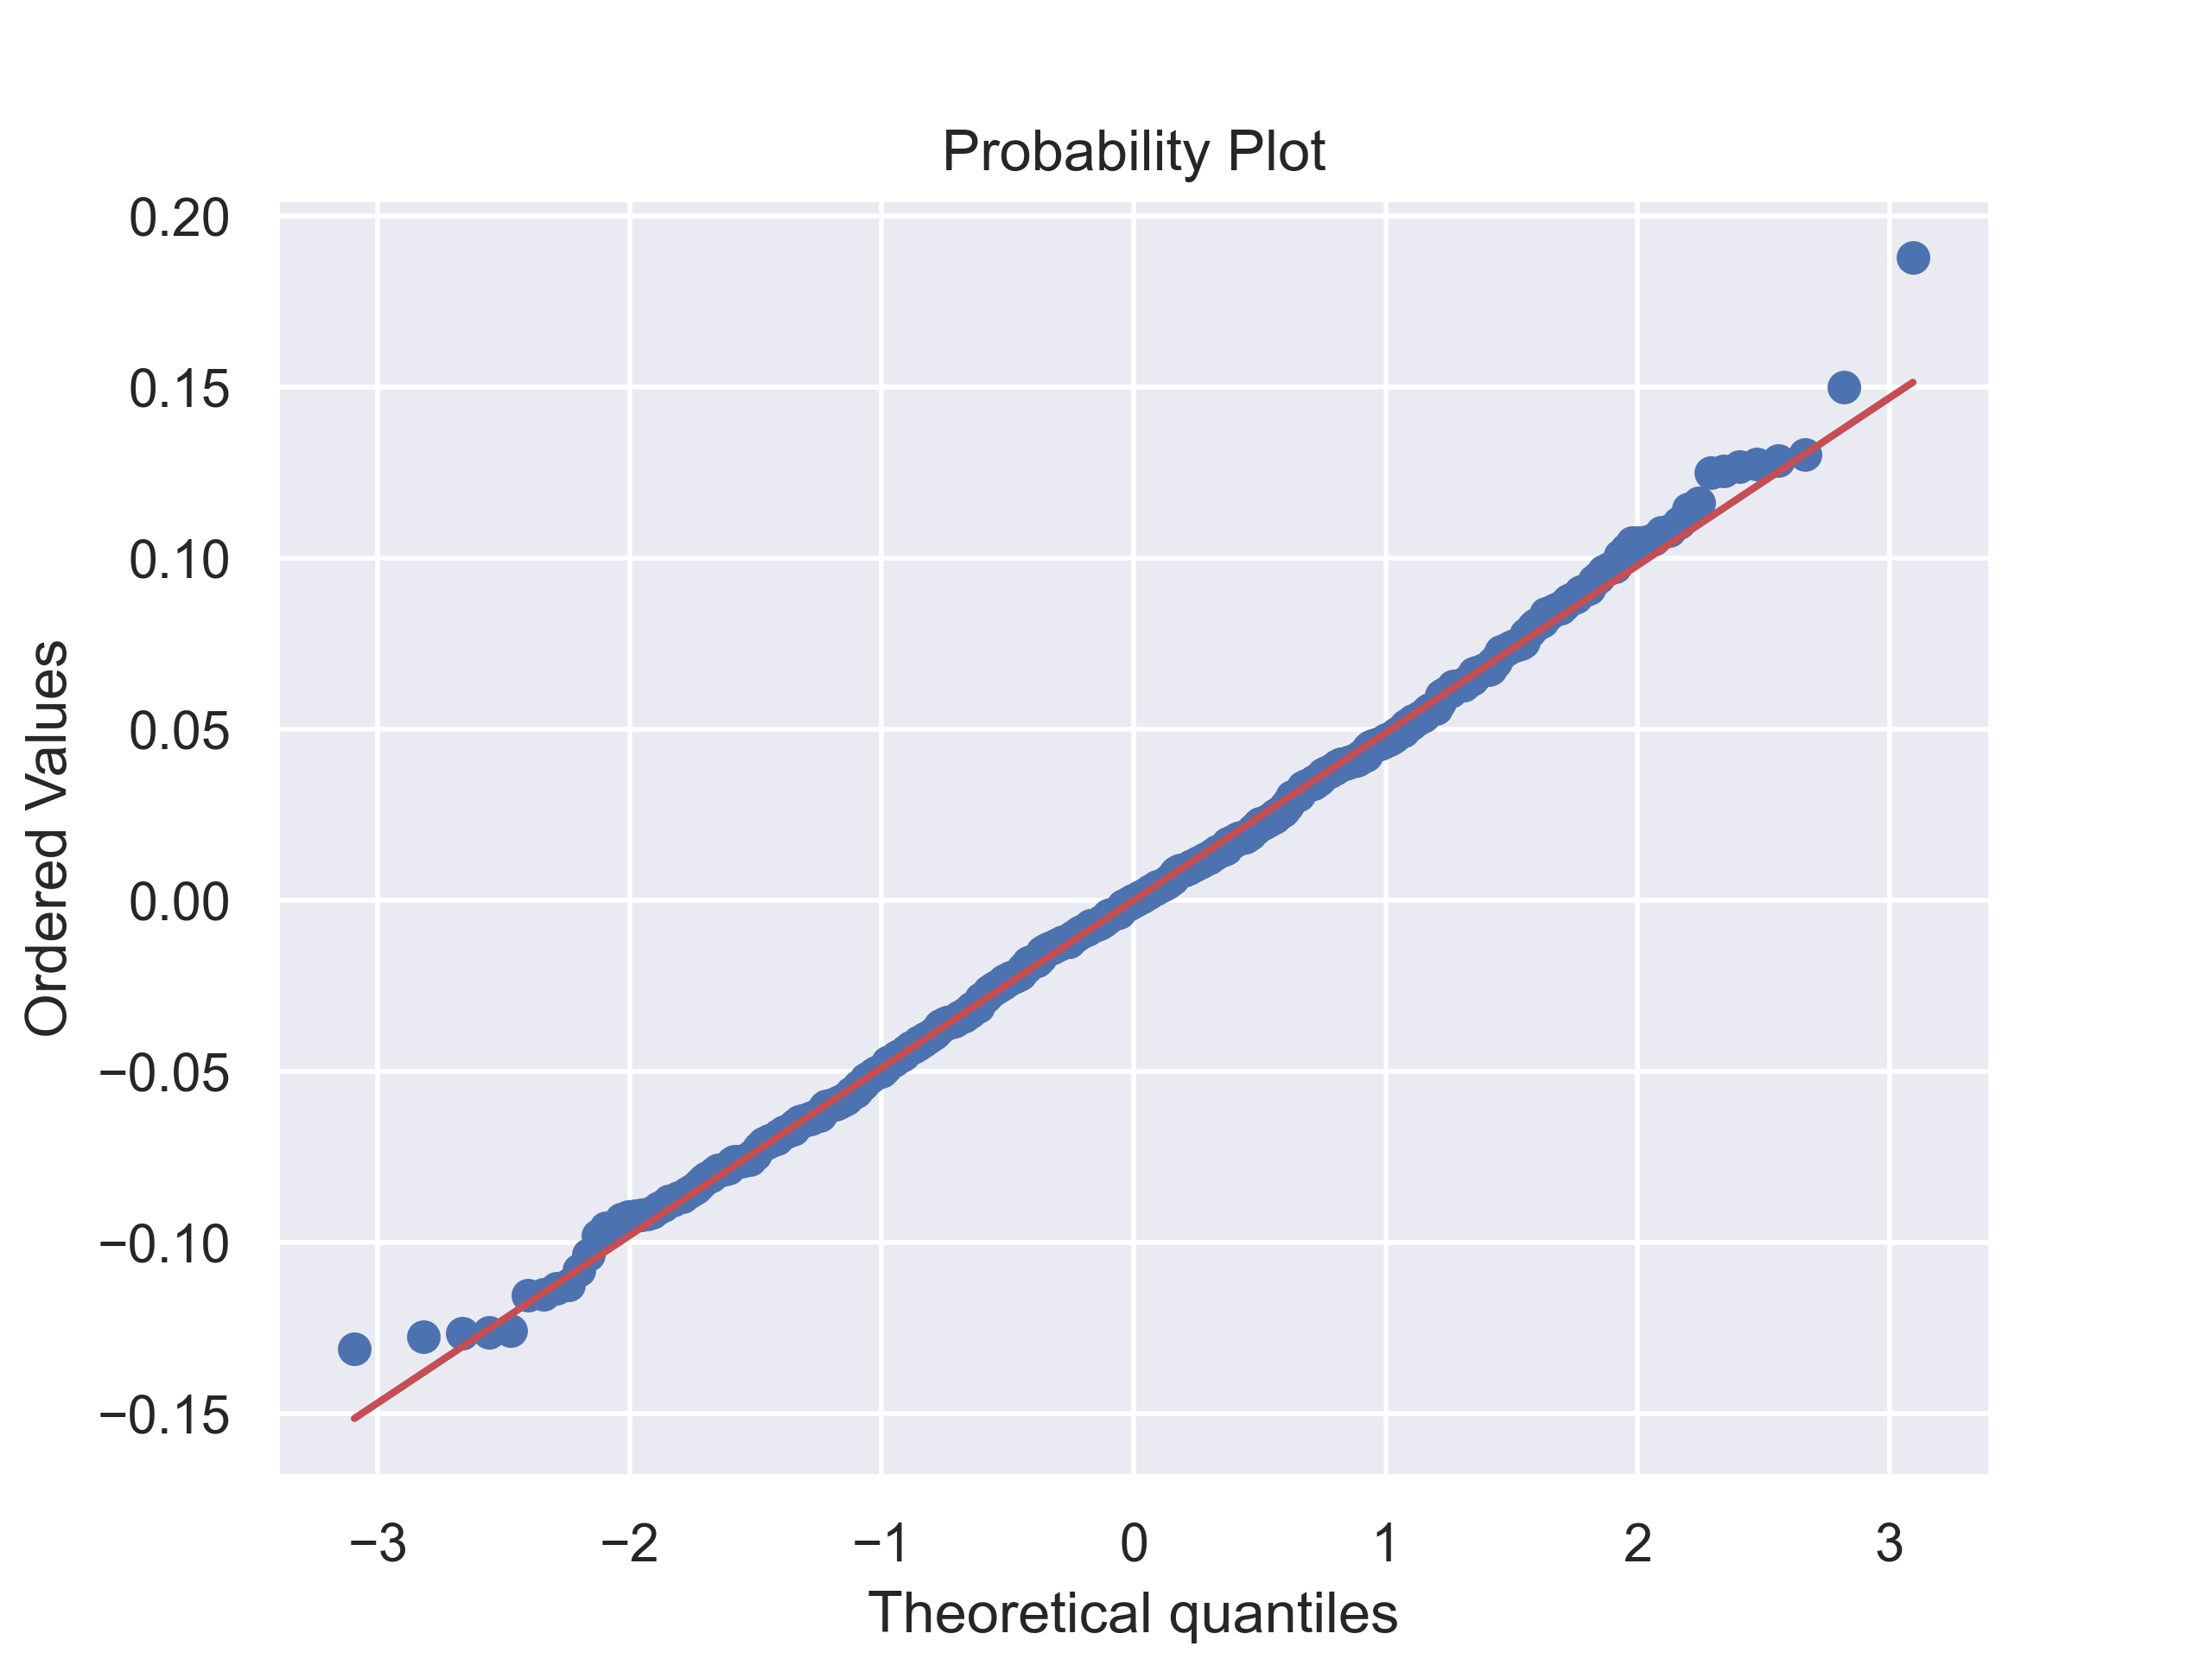
\includegraphics[width=\textwidth]{QQ_plot.png}
		\caption{Q-Q plot of residuals with respect to normal distribution.}
		\label{fig:}
	\end{subfigure}
	\caption{Check for normality of residuals}
	\label{fig: normality check}
\end{figure}
\begin{figure}[h]
	\centering
	\includegraphics[width=0.6\textwidth]{Fitted_Vs_Residual.png}
	\caption{Scatter plot of residual values against fitted values in the model }
	\label{fig:Fitted_Vs_Residual}
\end{figure}





\section{Actionable insights and Recommendations}
\subsection{Actionable insights}
\begin{itemize}
	\item Shows released on Saturday has  highest first day viewership followed by Wednesday, Sunday and the rest days.
	\item Shows released in summer have higher content views. 
	\item Presence of major sports event on the day of show release adversely affects viewership in all genres.
	\item In summer there is lesser chance of clash with a major sports event.
	\item  For each million visitors in the last week there are 0.129 million more content views when the show is released.
	\item There is significant correlation between trailer views and content views. For each million trailer views there are 0.0023 million more content views with very high confidence.
	\item The correlation between ad impression and content view is very small. This shows ad campaign has been ineffective.
	
\end{itemize}
  
\subsection{Business Recommendations}
\begin{itemize}
	\item To increse chance of viewership release new content on saturday.
	\item If there is an unavoidable sports event on the same day of release, it is advised to change the day of release.
	\item It is recommended to bring more content in summer probably because there is less chance of collision with sports event in summer and also there are vacations going on.  
	\item Take action to increase visitors on the OTT platform prior to a new show release. 
	\item Invest more in making impressive trailers. Find improved methods to increase trailer views prior to show release.
	\item Advertisements have been ineffective. Take necessary actions and consultations from ad department to increase influence of ads about new show release across different  platforms.
	\item The linear model described in this report can explain 75\% of the story in the content view data set. It may be used for prediction, planning and inferences.      
\end{itemize}
\begin{centering}
\vspace{20pt}
\subsection*{End of Report\\Submitted by : Haraprasad Dhal}
\end{centering}
\clearpage
\subsection{Appendix}
\small{\textbf{Trial of a model with log transformation of trailer views:}}\\
From figure \ref{fig:log_comparison} we observe that there is a resemblance of plot between trailer and content views to that of a logarithm plot. So we carried out a model where we took log transformation of trailer views variable. On figure \ref{fig:log_performance} we have shown the model performance. Since the values are not very different from the models where we did not take any transformations we did not proceed further with this model. Nevertheless, this log model also gives good result on training data similar to our final model. 
\begin{figure}[h]
		\centering
	\begin{subfigure}[t]{0.6\textwidth}
		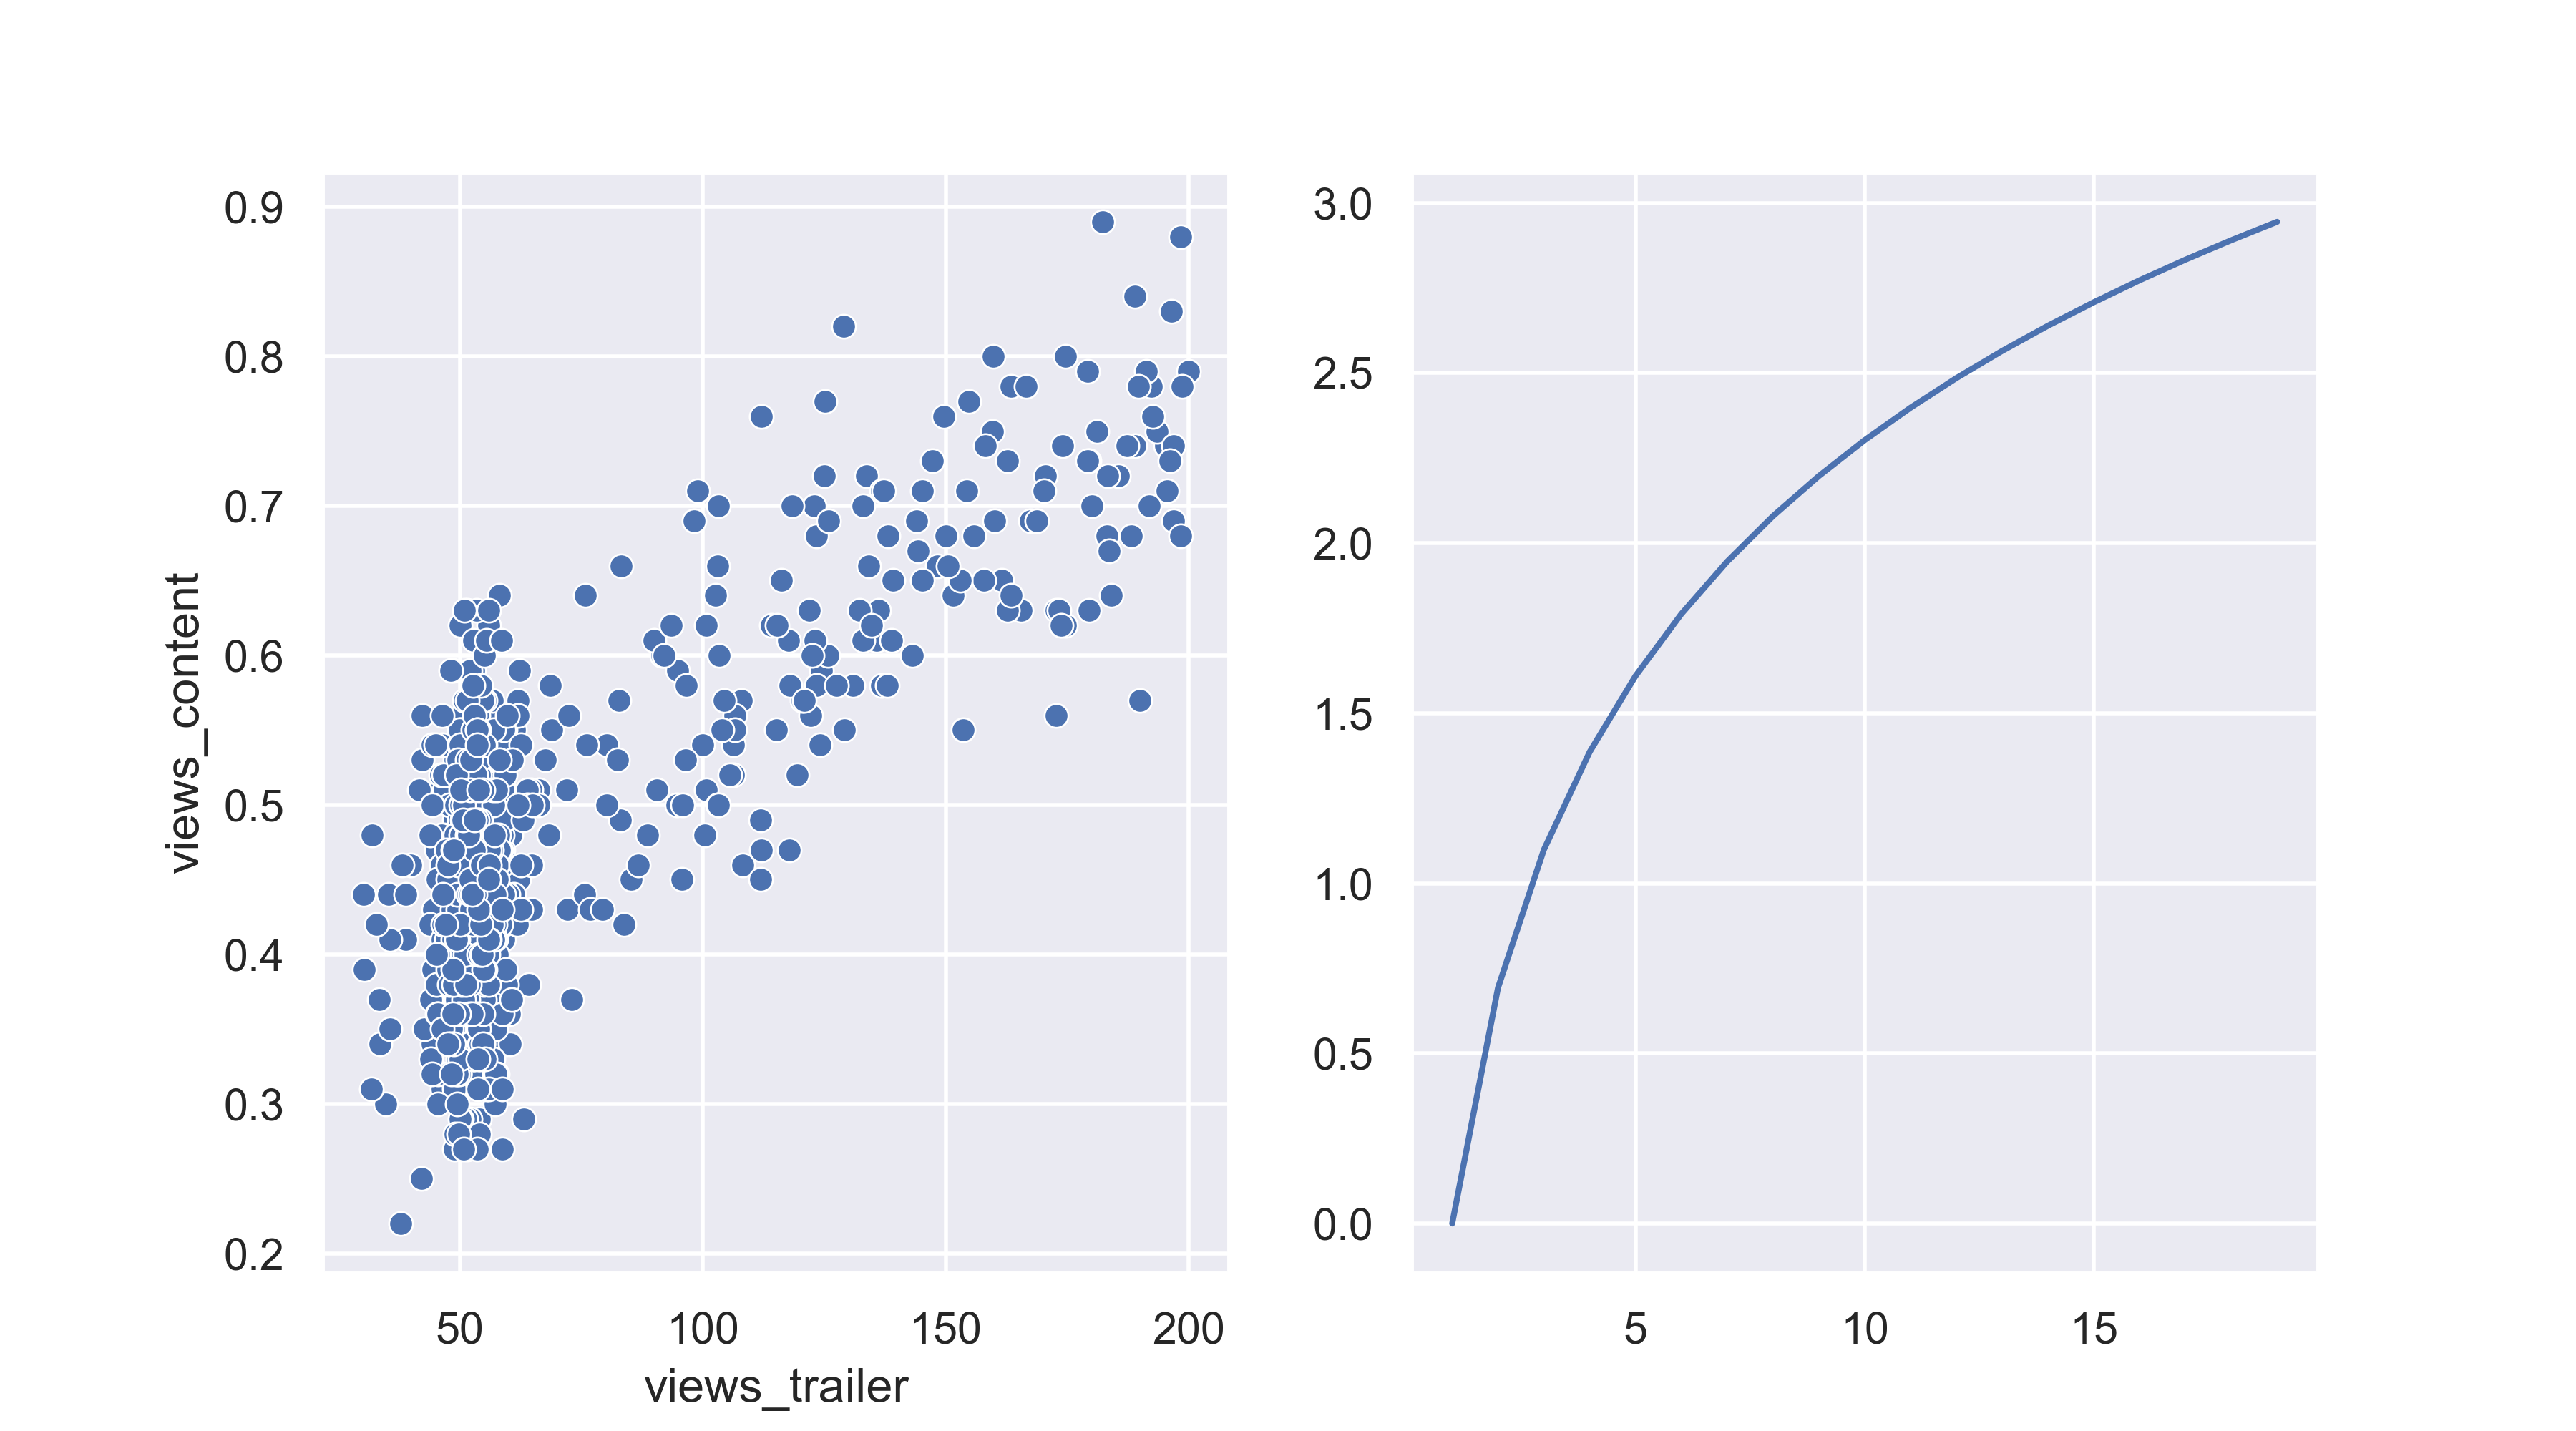
\includegraphics[width=\textwidth]{log_compare.png}
		\caption{Comparison of trailer views vs content views to log plot}
		\label{fig:log_comparison}
	\end{subfigure}
	\hfill
	\begin{subfigure}[t]{0.39\textwidth}
		\centering
		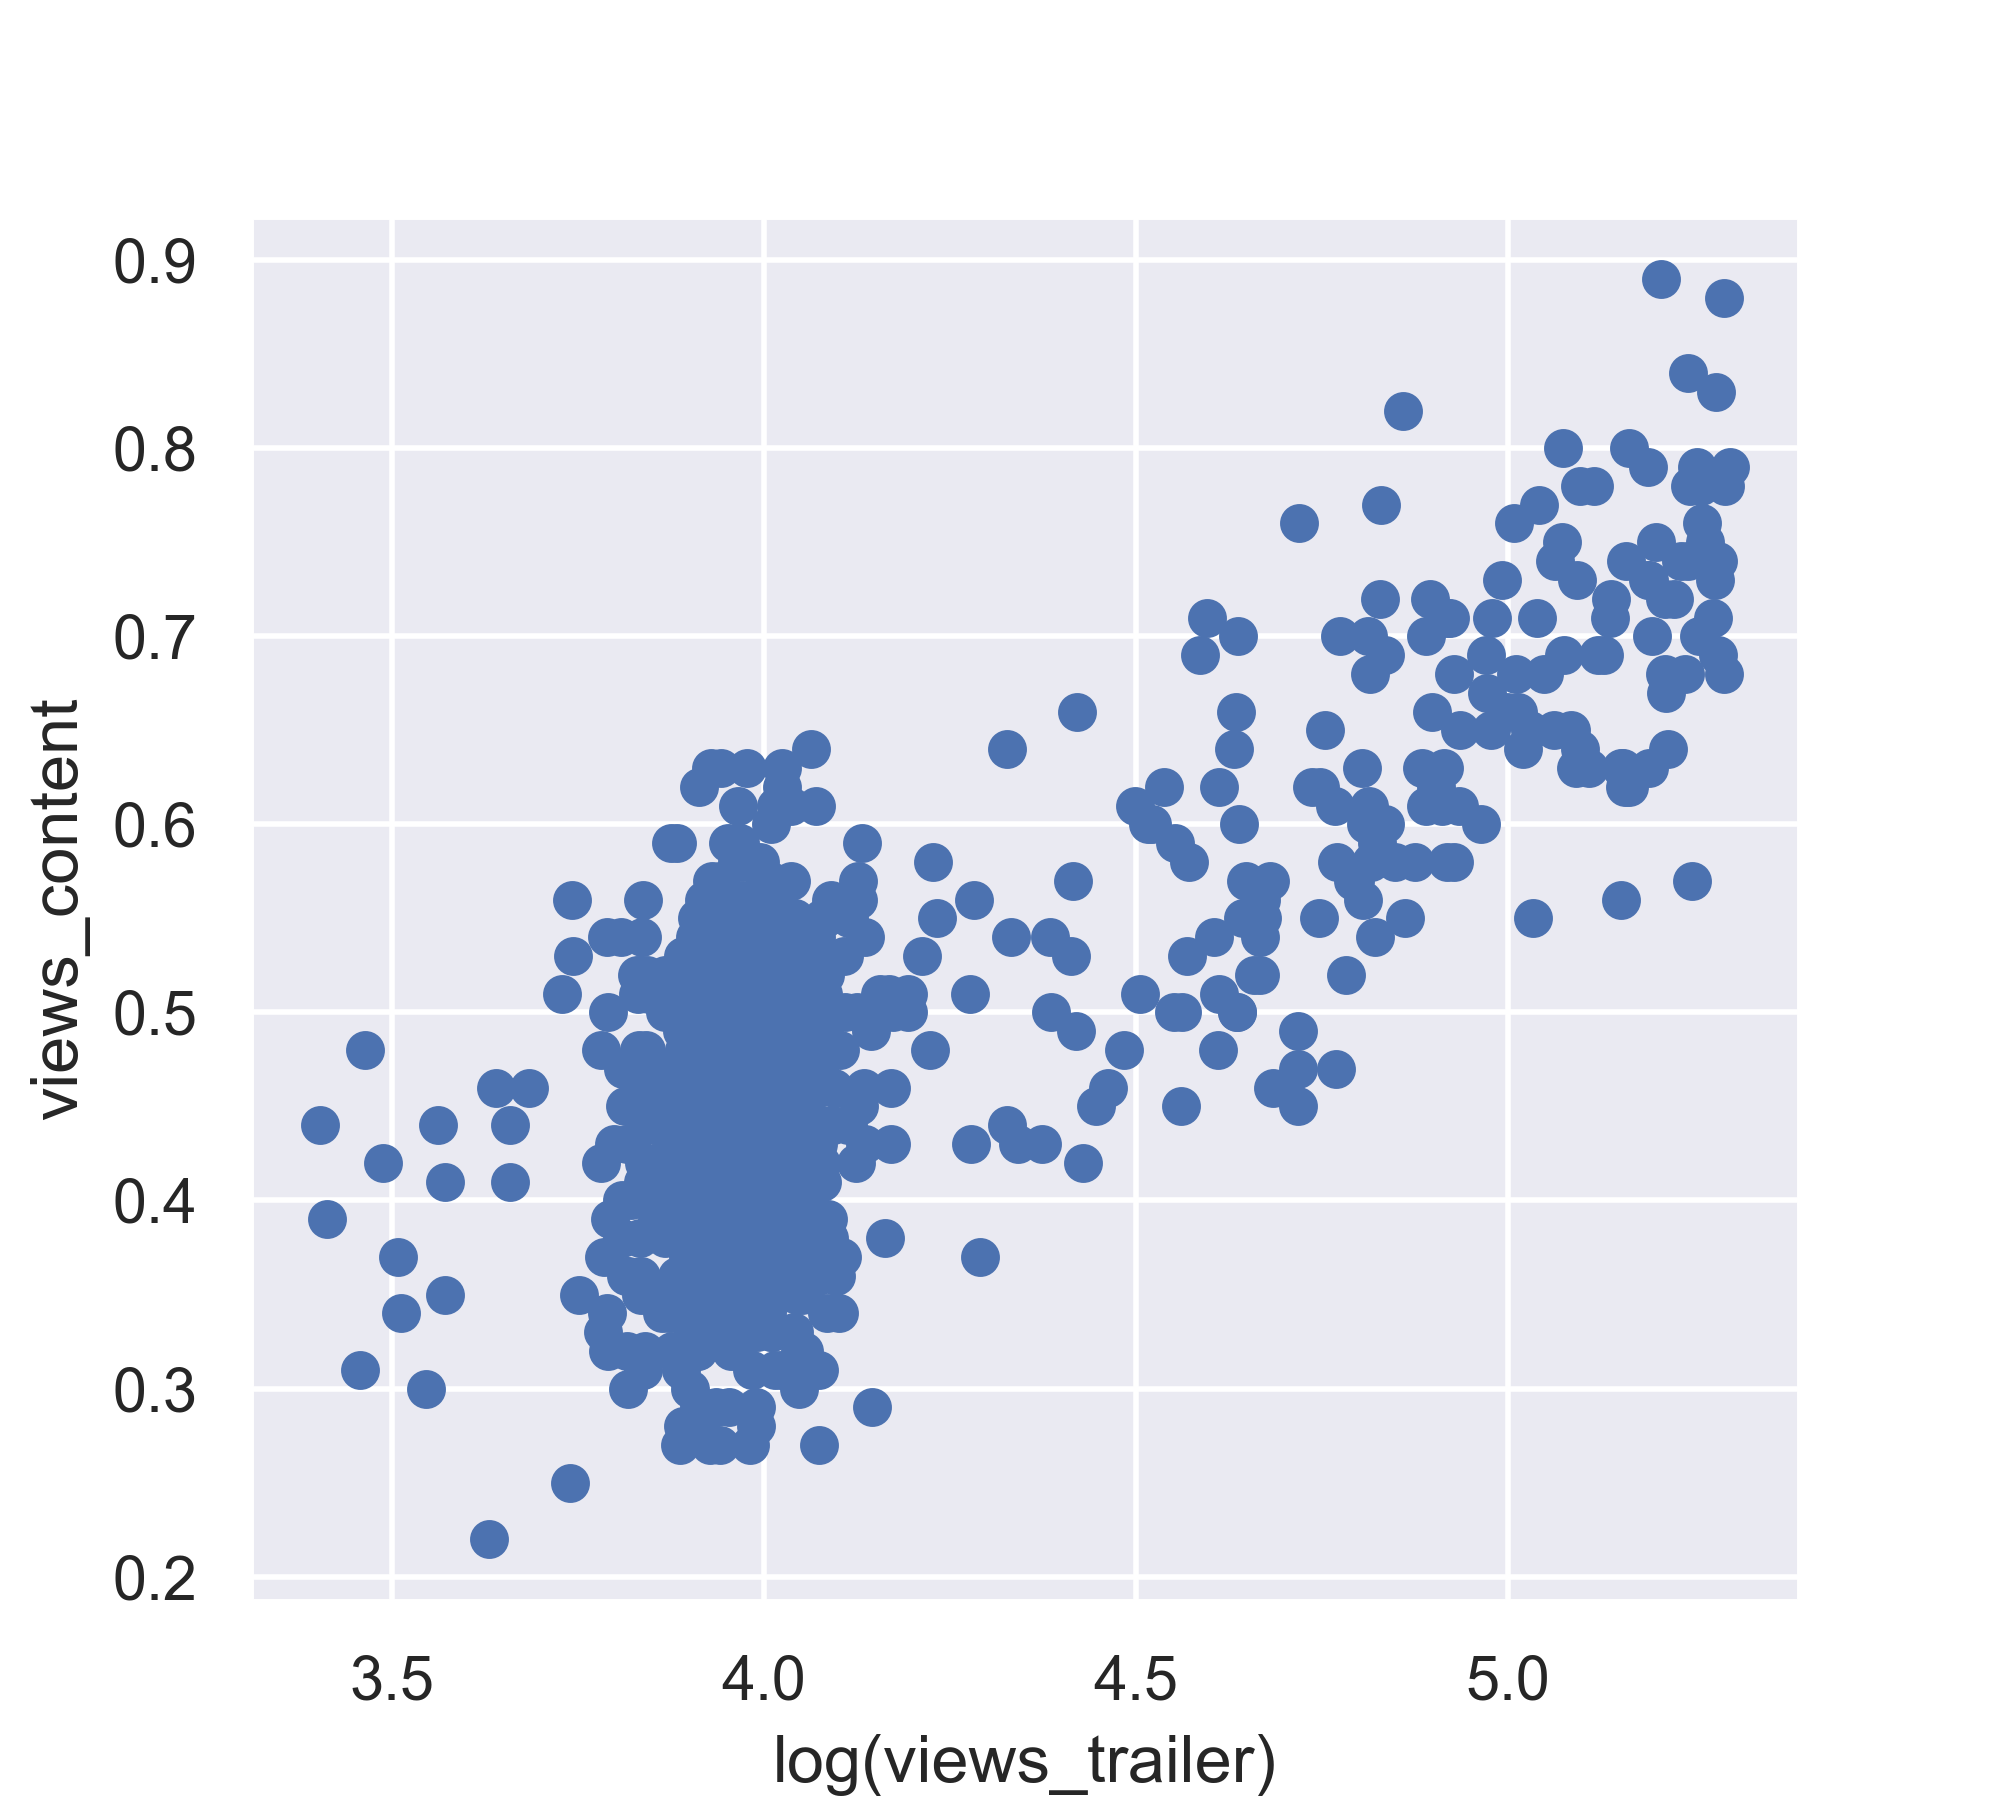
\includegraphics[width=\textwidth]{log_trailer.png}
		\caption{log(trailer views) vs content views scatter plot}
		\label{fig:log_trailer}
	\end{subfigure}
	\caption{A trial with taking log transformation}
	\label{fig:}
\end{figure}
\begin{figure}[h]
	\centering
	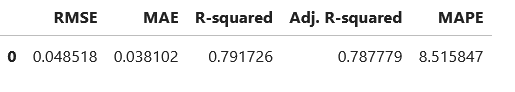
\includegraphics[width=0.7\textwidth]{log_model_performance.png}
	\caption{Model performance when we take log of trailer views}
	\label{fig:log_performance}
\end{figure}
\end{document}